%% !TEX program = xelatex
%%
%% This is file `thesis.tex',
%% generated with the docstrip utility.
%%
%% The original source files were:
%%
%% nudtpaper.dtx  (with options: `thesis')
%% 
%% This is a generated file.
%% 
%% Copyright (C) 2018 by TomHeaven <hanlin_tan@nudt.edu.cn>
%% 
%% This file may be distributed and/or modified under the
%% conditions of the LaTeX Project Public License, either version 1.3a
%% of this license or (at your option) any later version.
%% The latest version of this license is in:
%% 
%% To produce the documentation run the original source files ending with `.dtx'
%% through LaTeX.
%% 
%% Thanks LiuBenYuan <liubenyuan@gmail.com> for maintainence.
%% Thanks Xue Ruini <xueruini@gmail.com> for the thuthesis class!
%% Thanks sofoot for the original NUDT paper class!
%% 
%1. 规范硕士导言
% \documentclass[master,ttf]{nudtpaper}
%2. 规范博士导言
% \documentclass[doctor,twoside,ttf]{nudtpaper}
%3. 如果使用是Vista
% \documentclass[master,ttf,vista]{nudtpaper}
%4. 建议使用ttf字体
% \documentclass[doctor,twoside,fz]{nudtpaper}
%5. 如果想生成盲评，传递anon即可，仍需修改个人成果部分
% \documentclass[master,otf,anon]{nudtpaper}
%
\documentclass[master,ttf,twoside,prof]{nudtpaper}
\usepackage{mynudt}
\usepackage{multirow,array,makecell}
\usepackage{arydshln}
\usepackage{tikz}
\usetikzlibrary{positioning,arrows.meta,shapes.geometric,calc}
\raggedbottom
\setlength{\textfloatsep}{10pt plus 2pt minus 2pt}
\setlength{\floatsep}{8pt plus 2pt minus 2pt}
\setlength{\intextsep}{8pt plus 2pt minus 2pt}
\renewcommand{\topfraction}{0.9}
\renewcommand{\bottomfraction}{0.8}
\renewcommand{\textfraction}{0.07}
\renewcommand{\floatpagefraction}{0.8}

\classification{TP302.1}
\serialno{23023014}
\confidentiality{公开}
\UDC{004.8}
\title{面向异构 GPU 集群的多模态大语言模型\\并行训练技术研究}
\displaytitle{面向异构 GPU 集群的多模态大语言模型并行训练技术研究}
\author{范锦山}
\zhdate{\zhdigits{2026}年\zhnumber{4}月}
\entitle{Research on Parallel Training Techniques for Multimodal Large Language Models in Heterogeneous GPU Clusters}
\enauthor{Jinshan Fan}
\endate{April, 2026}
\subject{电子信息}
\ensubject{Computer Technology}
\researchfield{计算机技术}
\concretefield{并行智能计算}
\supervisor{李东升\quad{}研究员}
\cosupervisor{赖志权\quad{}副研究员}  % 协助指导教师，没有就空着
\ensupervisor{Prof. Dongsheng Li}
\encosupervisor{Associate Prof. Zhiquan Lai} % 协助指导教师英文，没有就空着
\papertype{工学}
\enpapertype{Engineering}
% 加入makenomenclature命令可用nomencl制作符号列表。
\AtBeginDocument{\makeatletter\let\origcleardoublepage\cleardoublepage\makeatother}

\begin{document}
	\graphicspath{{figures/}}
	% 制作封面，生成目录，插入摘要，插入符号列表 \\
	% 默认符号列表使用denotation.tex，如果要使用nomencl \\
	% 需要注释掉denotation，并取消下面两个命令的注释。 \\
	% cleardoublepage% \\
	% printnomenclature% \\
\maketitle
\frontmatter
\cleardoublepage
\tableofcontents
\cleardoublepage
\listoftables
\cleardoublepage
\listoffigures

\midmatter
\begin{cabstract}
多模态大语言模型（MLLM）融合视觉、语言等模态的感知与生成能力，是当前人工智能研究的重要方向，其训练依赖分布式与并行计算。实际部署中的 GPU 集群往往由多代、多型号设备混合组成，存在显存、算力与通信的异构；而 MLLM 在结构上由编码器、投影层与 LLM 骨干等异构模块组成，训练时又广泛采用分阶段冻结策略，导致各阶段计算与显存需求差异显著。现有并行策略（如 Megatron-LM、ZeRO）多假设同构集群与单一模型形态，在异构环境下易产生负载不均衡、资源利用率低及冻结场景下的冗余计算与通信等问题。

本文从流水线划分与调度、显存优化两个层面开展研究。在划分与调度方面，提出 MMoH 框架：通过需求驱动的设备拓扑识别、复合粒度模型抽象与冻结感知的整数规划划分，在给定异构集群与 MLLM 配置下自动生成与当前训练阶段相匹配的流水线并行策略；通过提前终止调度器在连续冻结阶段省略不必要的反向计算与阶段间通信，在保持收敛性的前提下提升吞吐。在显存优化方面，针对现有框架（如 Megatron-LM）中激活重计算采用全局统一配置、在异构集群上难以同时兼顾显存安全与计算效率的问题，提出 HR-MMoH 的异构激活重计算方法：系统梳理 Megatron 的重计算粒度与子模块配置参数，在 MMoH 划分基础上为各流水线阶段根据其显存上限与算力独立配置重计算粒度与子模块集合，显存紧张阶段采用更激进的检查点以降低 OOM 风险，显存充裕阶段采用较保守的配置以减少多余重算，并通过基于剖析的配置策略与 MMoH 形成“划分—调度—显存优化”的联合优化。在两种异构集群与两种规模 MLLM（3B、12B）上的实验表明，MMoH 在多种冻结场景下相对 Megatron-LM、Whale、Espresso 均可取得最高吞吐，最高可达约 1.77 倍加速，提前终止调度器可带来约 8\%--19\% 的额外增益；HR-MMoH 的按阶段差异化配置思路通过剖析实验得到验证，可为显存受限场景下的训练提供补充手段。本文为异构 GPU 集群上 MLLM 的高效并行训练提供了可参考的技术路径。
\end{cabstract}
\ckeywords{多模态大语言模型；异构 GPU 集群；流水线并行；激活重计算；MMoH}

\begin{eabstract}
Multimodal large language models (MLLMs) integrate vision, language, and other modalities for perception and generation, and have become a major focus of artificial intelligence research; their training relies on distributed and parallel computing. In practice, GPU clusters are often composed of mixed generations and models of devices, exhibiting heterogeneity in memory, compute, and communication. Meanwhile, MLLMs are architecturally composed of heterogeneous modules such as encoders, projectors, and LLM backbones, and training commonly adopts stage-wise freezing, leading to significant differences in compute and memory demand across pipeline stages. Existing parallel strategies (e.g., Megatron-LM, ZeRO) mostly assume homogeneous clusters and uniform model structure, which in heterogeneous settings can cause load imbalance, low resource utilization, and redundant computation and communication under freezing.

This thesis addresses the problem from two aspects: pipeline partitioning and scheduling, and memory optimization. For partitioning and scheduling, we propose the MMoH framework: it uses demand-driven device topology identification, multi-granularity model abstraction, and freeze-aware integer-programming-based partitioning to automatically generate pipeline-parallel strategies that match the current training stage for a given heterogeneous cluster and MLLM configuration; an early-termination scheduler omits unnecessary backward computation and inter-stage communication at consecutive frozen stages, improving throughput while preserving convergence. For memory optimization, we address the fact that existing frameworks (e.g., Megatron-LM) use a single global activation recomputation configuration, which is ill-suited to heterogeneous clusters where memory-tight stages may still hit OOM while memory-rich stages incur unnecessary recomputation. We propose HR-MMoH with heterogeneous-aware gradient checkpointing: we systematically summarize Megatron's recomputation granularity and submodule parameters, then assign each pipeline stage an independent recomputation configuration (granularity and submodule set) according to its memory headroom and compute, so that memory-tight stages use more aggressive checkpointing to reduce OOM risk and memory-rich stages use conservative settings to avoid redundant recomputation; a profiling-based configuration strategy is used and integrated with MMoH to form a joint ``partitioning--scheduling--memory optimization'' pipeline. Experiments on two heterogeneous clusters and two MLLM scales (3B and 12B parameters) show that MMoH achieves the highest throughput under various freezing scenarios compared with Megatron-LM, Whale, and Espresso, with speedups of up to about 1.77$\times$, and the early-termination scheduler brings an additional 8\%--19\% gain; the per-stage heterogeneous checkpoint configuration in HR-MMoH is validated via profiling and provides a complementary means for memory-constrained training. This work provides a practical technical path for efficient parallel training of MLLMs on heterogeneous GPU clusters.
\end{eabstract}
\ekeywords{Multimodal large language model; Heterogeneous GPU cluster; Pipeline parallelism; Gradient checkpointing; MMoH}

\cleardoublepage
% TeX
\chapter{本文中英文对照表}

表~\ref{tab:appendix-bilingual} 给出正文常用术语的中英文对照；第二列在必要时附缩写或原文记号。

\begingroup
\small
\setlength{\LTpre}{6pt}
\setlength{\LTpost}{6pt}
\renewcommand{\arraystretch}{1.12}
\begin{longtable}{@{}p{5.6cm}p{7.4cm}@{}}
	\caption{本文主要术语中英文对照表}\label{tab:appendix-bilingual} \\
	\toprule
	\textbf{中文} & \textbf{英文} \\
	\midrule
	\endfirsthead
	\multicolumn{2}{@{}l@{}}{\small 续表~\thetable} \\
	\toprule
	\textbf{中文} & \textbf{英文} \\
	\midrule
	\endhead
	\midrule
	\multicolumn{2}{r@{}}{\small 续下页} \\
	\endfoot
	\bottomrule
	\endlastfoot
	% --- 第 1 章：基础概念与模型 ---
	自注意力机制 & Self-Attention \\
	深度神经网络 & Deep Neural Network (DNN) \\
	卷积神经网络 & Convolutional Neural Network (CNN) \\
	循环神经网络 & Recurrent Neural Network (RNN) \\
	计算机视觉 & Computer Vision (CV) \\
	自然语言处理 & Natural Language Processing (NLP) \\
	语音识别 & Speech Recognition (SR) \\
	大语言模型 & Large Language Model (LLM) \\
	多模态大语言模型 & Multimodal Large Language Model (MLLM) \\
	通用人工智能 & Artificial General Intelligence (AGI) \\
	迁移学习 & Transfer Learning \\
	少样本学习 & Few-Shot Learning \\
	零样本学习 & Zero-Shot Learning \\
	扩展定律 & Scaling Laws \\
	图文对比学习CLIP & Contrastive Language-Image Pre-Training\\
	
	最优先进水平 & state-of-the-art (SOTA) \\
	% --- 第 1--2 章：MLLM 结构 ---
	模态编码器 & Modality Encoder \\
	输入投影层 & Input Projector \\
	LLM 基座 & LLM Backbone \\
	输出投影层 & Output Projector \\
	模态生成器 & Modality Generator \\
	扩散模型 & diffusion model \\
	模块异构 & module heterogeneity \\
	% --- 第 2 章：训练阶段与数据 ---
	模态对齐 & modality alignment \\
	指令微调 & instruction tuning \\
	% --- 并行、通信与显存 ---
	数据并行 & data parallelism (DP) \\
	分布式数据并行 & Distributed Data Parallel (DDP) \\
	张量并行 & tensor parallelism (TP) \\
	流水线并行 & pipeline parallelism (PP) \\
	序列并行 & sequence parallelism (SP) \\
	上下文并行 & context parallelism (CP) \\
	专家并行 & expert parallelism (EP) \\
	混合专家 & Mixture of Experts (MoE) \\
	混合并行 & hybrid parallelism\\
	微批次 & micro-batch \\
	小批量 & mini-batch \\
	一前向一反向调度 & One-Forward-One-Backward (1F1B) \\
	全归约 & AllReduce \\
	全收集 & All-Gather \\
	归约分散 & Reduce-Scatter \\
	全对全通信 & All-to-All \\
	点对点通信 & Peer-to-Peer (P2P) \\
	参数服务器 & parameter server \\
	流水级 & pipeline stage \\
	流水线气泡 & pipeline bubble \\
	混合精度训练 & mixed-precision training \\
	全分片数据并行 & Fully Sharded Data Parallel (FSDP) \\
	零冗余优化器 & Zero Redundancy Optimizer (ZeRO) \\
	环形注意力 & Ring Attention \\
	激活/激活值 & activation \\
	显存溢出 & Out Of Memory (OOM) \\
	负载均衡 & load balancing \\
	剖析/性能剖析 & profiling \\
	设备拓扑 & device topology \\
	整数规划 & integer programming \\
	复合粒度（模型抽象） & multi-granularity model abstraction \\
	成本模型 & cost model \\
	服务等级目标 & Service Level Objective (SLO) \\
	模型算力利用率 & Model FLOPs Utilization (MFU) \\
	% --- 框架与代表性系统（第 1--2 章） ---
	虚拟工作节点 & Virtual Worker (VW) \\
	剖析器 & Profiler\\
	GPU 分配器 & GPU Allocator \\
	阶段放置器 & Stage Placer \\
	全部重计算 & full recomputation \\
	选择重计算 & selective recomputation \\
	细粒度重计算 & fine-grained recomputation \\
	Top-$k$专家路由 & Top-$k$ (expert routing) \\
\end{longtable}
\endgroup

% \input{data/denotation}
\mainmatter
\setcounter{page}{1}
\renewcommand\UrlFont{\timesnr}

\chapter{绪论}

\section{研究背景与意义}
\label{sec:chap1-background}

\subsection{多模态大语言模型的训练}

深度神经网络（Deep Neural Network, DNN）在计算机视觉（Computer Vision, CV）、自然语言处理（Natural Language Processing, NLP）、语音识别（Speech Recognition, SR）等众多前沿领域取得了显著成效，近年来逐步成为众多关键前沿技术的核心基础\cite{galvatron2022}。
2017 年，Vaswani 等人提出基于自注意力机制（Self-Attention）的 Transformer 架构%
\cite{vaswani2017}，
摒弃了传统的循环神经网络（Recurrent Neural Network, RNN）与卷积神经网络（Convolutional Neural Network, CNN）结构，由于其适合并行计算且擅长捕捉长上下文信息，Transformer 架构迅速成为自然语言处理与跨模态建模等领域的主流模型结构。

在自然语言处理领域，基于 Transformer 的预训练大语言模型（Large Language Models, LLMs）持续刷新多项基准测试的成绩，并推动模型能力由特定任务优化向通用知识学习演进。
以 BERT\cite{bert} 为代表的带掩码的双向编码预训练范式在语言理解任务中取得了突出效果，与此同时，GPT-2\cite{gpt2}、T5\cite{t5} 所采用的自回归（Autoregressive）与编码器-解码器（Encoder-Decoder）机制在文本生成场景中展现出更强的能力。
随着模型规模进一步扩展，GPT-3\cite{brown2020gpt3} 及后续 GPT-4\cite{openai2023} 在少样本（Few-Shot）与零样本（Zero-Shot）条件下呈现出极强的语言表达与任务迁移能力。

在计算机视觉领域，Transformer 架构也取代了传统的卷积神经网络，成为视觉模型的主流选择。Vision Transformer（ViT）\cite{vit2020} 及其规模化扩展工作\cite{scaling_vit} 表明，图像经块划分后输入 Transformer 层进行特征提取，可在 ImageNet 等基准数据集上达到并在部分配置下超越传统卷积神经网络的性能。
由此可见，Transformer 架构具备跨模态扩展的能力，其适用范围并不局限于文本建模。

随着单模态模型的能力已经接近甚至超越人类水平，将语言、视觉、音频、表格等多模态信息纳入统一的模型框架进行联合表示与计算，成为当前学术界和工业界研究的热点，这种可以同时处理两种或两种以上模态信息的能力被称为多模态（Multimodality）。
在机器学习与人工智能中，常见模态包括文本、图像、视频、音频、表格以及各类传感器数据，这种多种模态的信息更接近人类接触到的复杂信息。
多模态大语言模型（Multimodal Large Language Models, MLLMs）是指在原有大语言模型的基础上，增加对图像、声音等其它模态的感知与生成能力的一类模型%
\cite{blip2,llava2023,flamingo2022}。
MLLMs 的先驱工作 CLIP\cite{clip2021}（Contrastive Language-Image Pre-Training）通过使用图像文本对进行训练，使模型拥有理解并描述图片的能力，DALL-E\cite{dalle2021} 则与 CLIP 相反，展示了从文本生成图像的可行性。

近年来，MLLMs 在架构与训练范式上发展迅速。
BLIP-2\cite{blip2} 提出 Q-Former 连接冻结的视觉编码器模型与 LLM 基座模型进行训练；
InstructBLIP\cite{instructblip2023} 在此基础上加强了视觉信息的提取能力，在多项零样本任务上取得 SOTA 结果；
LLaVA\cite{llava2023} 与 LLaVA-1.5\cite{llava15_2023} 采用简单线性投影层实现视觉与语言模态对齐，验证了轻量的连接器与大语言模型组合方案的有效性；
Qwen-VL\cite{qwenvl2023}、InternVL\cite{internvl2024} 等系列多模态大语言模型则进一步在长上下文、高分辨率与多图理解上扩展了模型能力。
这类模型既保留传统 LLMs 在语言理解、推理与生成上的强大能力，又能够直接处理图像、音频等多模态输入，实现跨模态交互与推理任务，因而被广泛认为是通往通用人工智能（Artificial General Intelligence, AGI）的最有前景的技术手段\cite{minigpt4,mllm_survey_acl2024}。

从功能表现来看，MLLMs 可完成图像描述、视觉问答、图文对话、文档理解，以及基于文本的图像或视频生成等复杂任务，在自动驾驶、智能助手等应用场景中具有极大应用价值。
在垂直领域，MLLMs 已延伸至医疗影像理解\cite{medical_vlm2024}等。
多模态大语言模型的相关评估常使用 VQAv2\cite{vqav2}、GQA\cite{gqa2019}、MMMU\cite{mmmu_benchmark2024} 等多模态基准，不断更新的基准测试也对模型规模与训练数据提出了更高要求。
从结构上看，MLLMs 通常包含以下核心组件，如图~\ref{fig:mllm_components} 所示：
（1）Modality Encoder，负责将图像、视频等非文本输入编码为特征表示，常采用预训练的视觉模型（如 CLIP、ViT）；
（2）Input Projector，负责将编码后的多模态特征映射到与 LLM 词嵌入对齐的语义空间，常见形式包括线性层、Q-Former\cite{blip2} 等轻量级模块；
（3）LLM Backbone，即大语言模型主体，承担主要的内容理解与生成任务，处于 MLLMs 架构的核心地位，多模态能力通常是在其基础上的扩展与增强；
（4）Output Projector（在需要多模态生成时），将 LLM 输出映射到与目标模态生成器对齐的表示空间；
（5）Modality Generator（在需要多模态生成时），负责生成图像、音频等目标模态，常采用扩散模型（如 Stable Diffusion）等。

\begin{figure}[htbp]
  \centering
  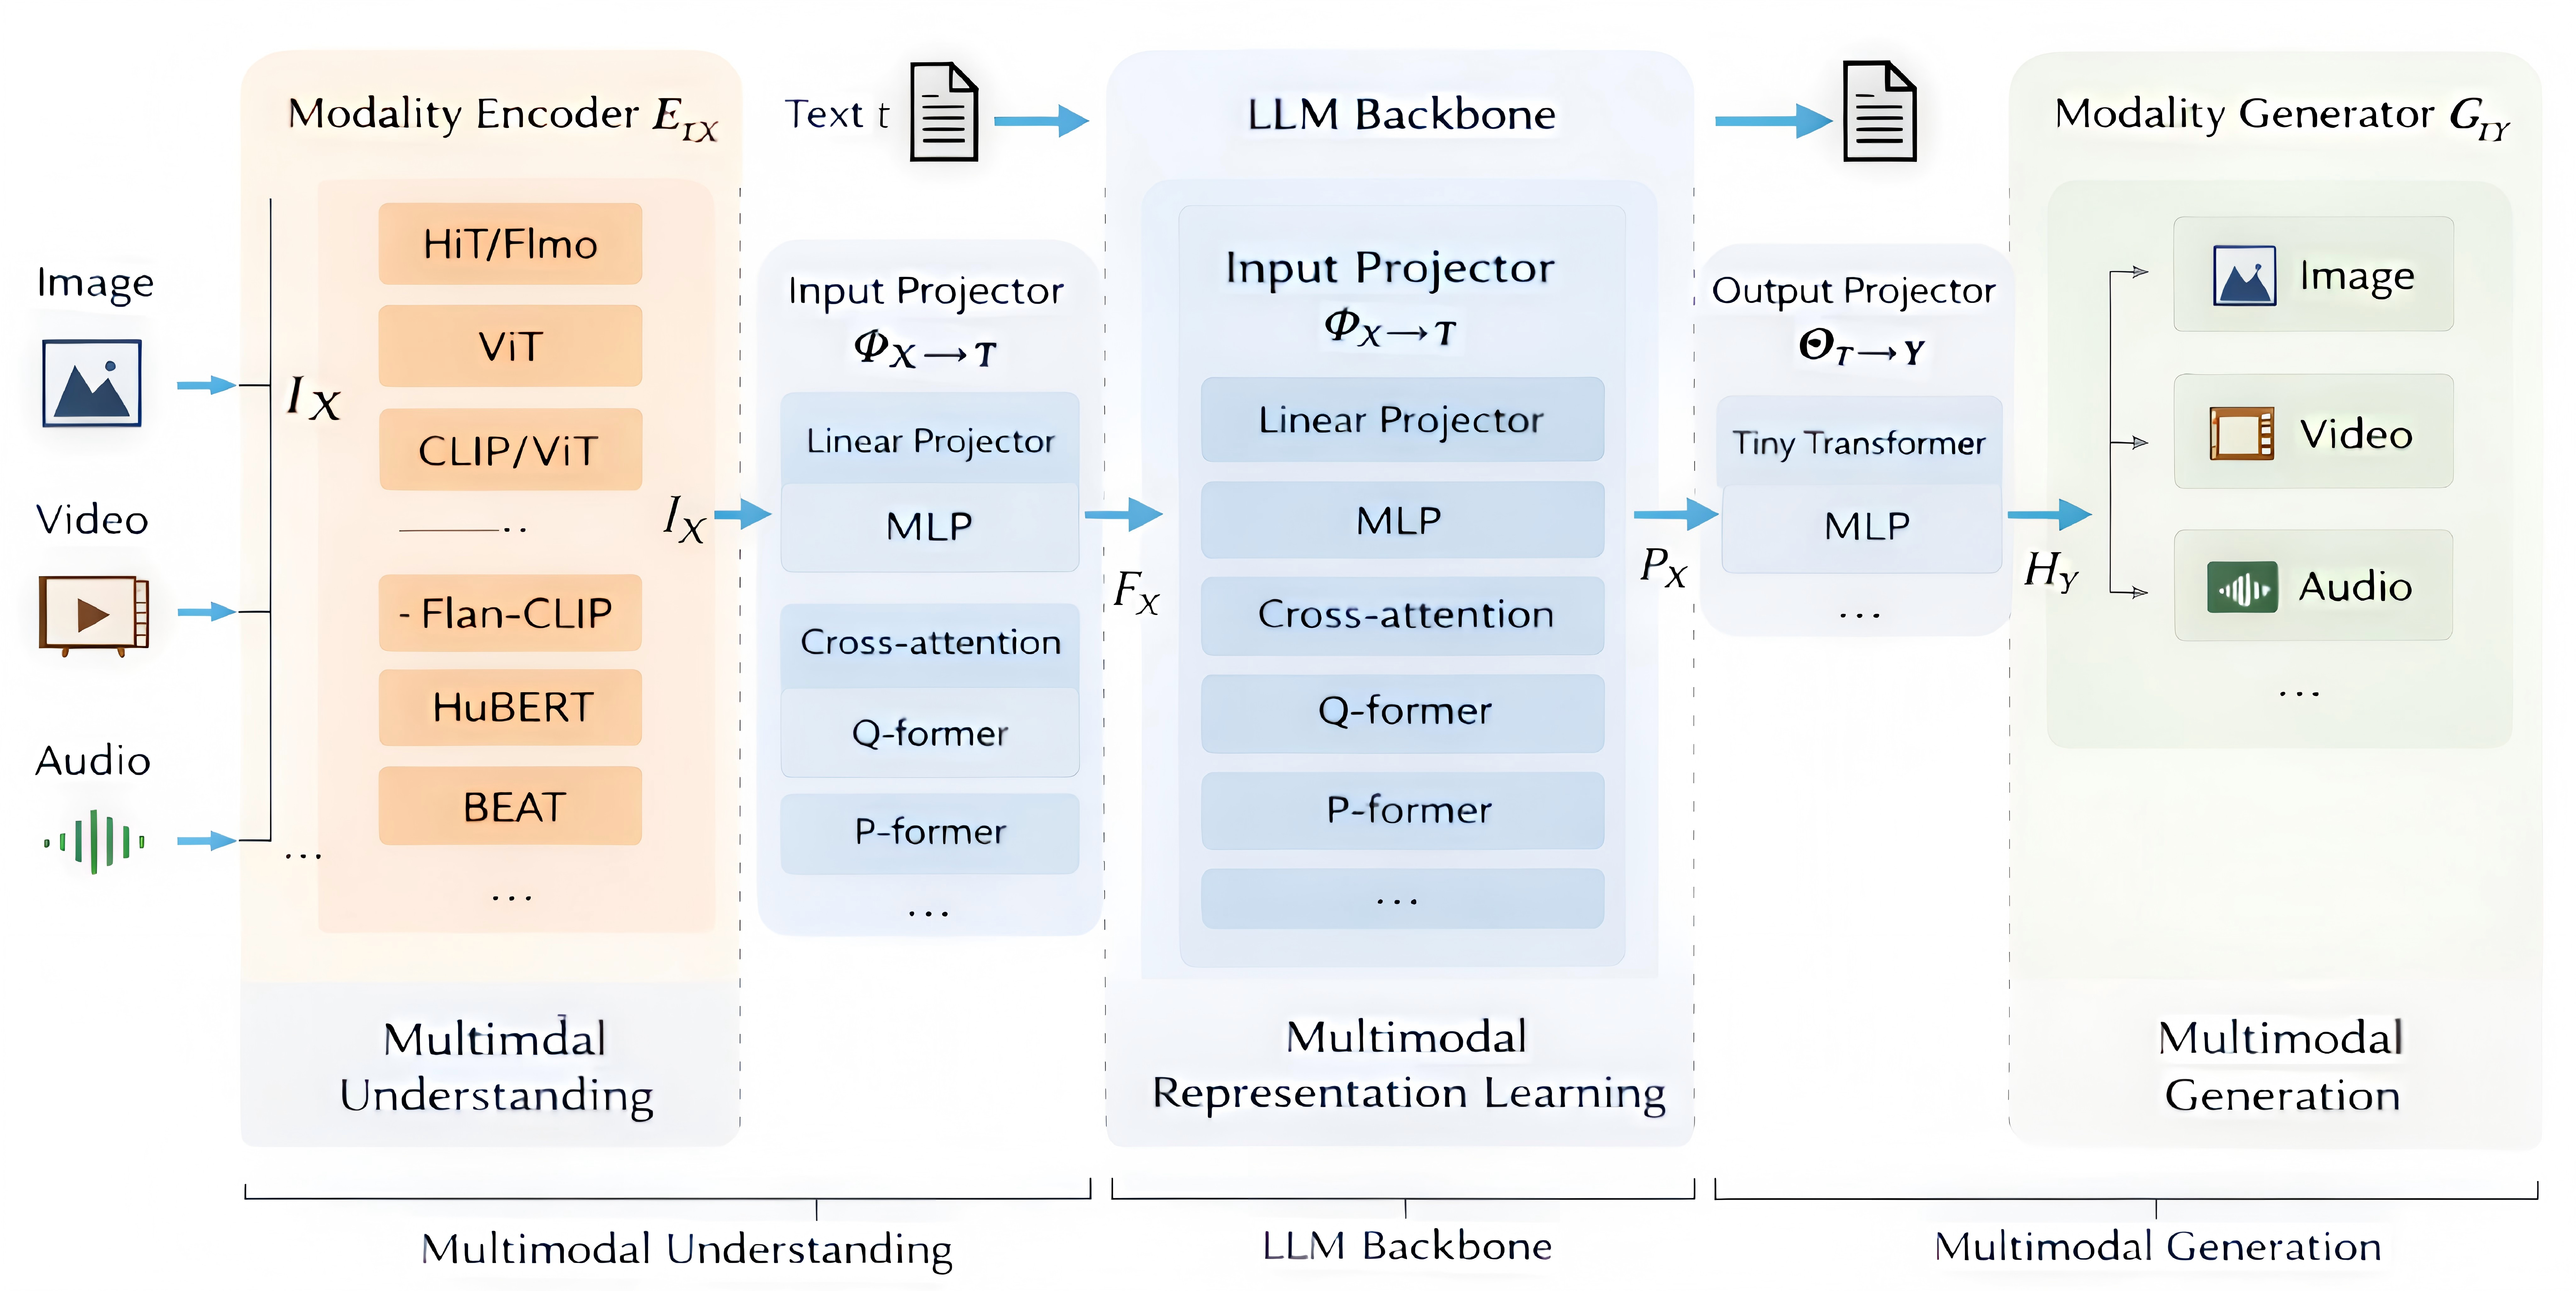
\includegraphics[width=\linewidth]{mllm_components.pdf}
  \caption{多模态大语言模型的核心组成部分}
  \label{fig:mllm_components}
\end{figure}

多模态大语言模型能力的拓展既依赖上述编码器、投影层、基座模型与可选生成器等模块的协同设计，也依赖参数与数据规模的提升。
参数和数据规模决定了模型可达的效果上限，而多模块的协同设计则影响模型的训练过程。
在大语言模型占据主体参数量的架构下，针对 LLMs 总结出的扩展定律（Scaling Laws）与数据规模规律，同样深刻影响着 MLLMs 训练的资源需求。
已有实证研究表明，模型性能通常会随参数规模与训练数据规模的增加而稳定提升，这一现象被总结为“扩展定律”（Scaling Laws）\cite{kaplan2020scaling}。
为追求更强性能，工业界与学术界不断推出参数量更大、数据规模更大的模型，
从数亿参数（如 BERT）到千亿、万亿参数（如 GPT-3、Gopher\cite{gopher2022}、DeepSeek-V3\cite{deepseek2024}、Qwen2.5\cite{qwen2024}、
LLaMA 2/3\cite{llama2_2023,llama3}、Gemma\cite{gemma2024}、Mistral\cite{mistral2023} 等开源与闭源 LLMs），
单卡或单机 GPU 的显存与算力已无法容纳模型的完整训练流程%
\cite{megatron2021,megatron2020}。
相应地，多模态大语言模型的预训练与指令微调所需的数据量也急剧增长，从数百万图文对到数十亿级样本，单机的运算速度已经远远无法满足企业对模型迭代速度的需求。
不仅如此，长上下文与多模态联合基准\cite{long_context_benchmark2024} 的普及进一步推高了对训练规模与效率的需求。
在上述参数规模与数据规模的限制下，单个计算设备的显存与算力均难以独立支撑完整的训练流程，因此必须借助分布式并行训练技术，将模型参数、优化器状态、激活值与数据分散至多台设备，通过节点间的通信协同完成多模态大语言模型的训练%
\cite{zero2020,zero2021}。

目前，支撑大规模 MLLMs 训练的主流手段包括数据并行、张量并行、流水线并行、序列与专家并行等多维混合并行技术\cite{pytorch_ddp,megatron2020,megatron2021,gpipe,pipedream2019,gshard}，以及面向参数与优化器状态的 ZeRO 系列显存分片技术\cite{zero2020,zero2021}；上述策略常与混合精度训练\cite{mixed_precision2018}、Flash Attention\cite{flash_attention_2022,flashattention3_2024} 等相结合，共同支撑当前大规模模型训练任务。
在采用上述并行策略的同时，训练过程仍面临较大的显存压力。
由于前向传播中需要保存中间激活以供反向传播时计算梯度使用，中间激活的显存占用随序列长度近似指数增长，在单设备上常构成主要显存压力，从而限制模型训练的上下文长度，进而限制模型能力上限。
ZeRO 等分片技术主要缓解参数与优化器状态的显存占用，对单设备上激活占用的降低有限。
为此，重计算（亦称梯度检查点）通过在前向传播中丢弃中间激活、在反向传播时重算，以额外前向计算换取显存空间，使模型在相同硬件条件下能够采用更大批次或更长序列进行训练\cite{chen2016checkpoint,megatron2023}。
由于如今的模型训练上下文迅速增长，重计算成为当前大规模训练的显存优化关键技术，因此 Megatron-LM、DeepSpeed 等主流并行训练框架均支持重计算技术。

然而，上述策略在设计时多假设集群同构且模型是单一 Transformer 层堆叠的语言模型，其划分粒度、负载均衡与重计算策略均围绕“各模型层计算与显存相对均匀”这一前提展开。
对于 MLLMs 而言，会引入两个额外问题：其一是模型结构异构，MLLMs 各子模块在算子类型、参数量与激活体积上差异显著。
编码器以卷积或 ViT 块为主，投影层参数量较小，而 LLM 基座由大量同构 Transformer 层堆叠且占据绝大部分参数。这种异构性使得传统基于“按层均分”假设的模型划分方案难以适用。
其二是分阶段冻结导致的动态负载变化。
当某一模块被冻结时，其反向传播计算开销与优化器状态的显存开销显著下降，各模块的计算与显存占比随阶段切换而动态变化。
例如，在冻结编码器阶段，编码器侧的显存与计算负载骤减，而 LLM 基座承担大部分梯度计算，切换到冻结 LLM 阶段后，负载分布又会发生变化。
这种动态变化特性使得固定的模型划分配置难以在全训练流程中保持高效。

\subsection{异构 GPU 集群下的并行训练}

多模态大语言模型的训练效率与成本高度依赖底层硬件平台。
目前，工业界与学术界普遍采用 NVIDIA GPU 作为 MLLMs 训练的主要加速器，并通过多卡、多机集群进行分布式训练。
人工智能的快速发展也推动了硬件迭代的速度，大约每 1--2 年，NVIDIA 就会推出使用新一代计算架构的多款不同定位的 GPU，这给 MLLMs 的训练带来了新的挑战。

图~\ref{fig:nvidia_gpu_evolution} 描述了近年来 NVIDIA GPU 的架构演进。
2016--2017 年的 Pascal 计算架构（如 NVIDIA P100）与 Volta 计算架构（NVIDIA V100）奠定了数据中心 GPU 与 Tensor Core 的基础。
2018 年 Turing 架构（RTX 20 系）引入消费级光追与 INT8 推理。
2020 年 Ampere 架构推出 A100（40GB/80GB HBM2e）与消费级 RTX 30 系列（如 RTX 3090 24GB），支持 PCIe 4.0 与 NVLink 3.0，成为当前许多实验室与云平台的主力\cite{nvidia_a100}。
2022 年搭载 Hopper 架构的 H100（80GB/96GB HBM3）针对大语言模型训练做了专门优化\cite{nvidia_h100}，并广泛配备 NVLink 4.0 与 NVSwitch，单机多卡带宽可达数百 GB/s，
同年 Ada Lovelace 架构的 RTX 40 系列（如 RTX 4090 24GB）在消费级市场提供高性价比算力。
2024 年起，Blackwell 架构的 B100/B200 等数据中心 GPU 逐步量产，采用 HBM3e、更高带宽第五代 NVLink 与 PCIe 6.0，进一步拉大与旧代设备的性能与互联差距。
据 NVIDIA 在 GTC 等场合公开发布的产品路线图\cite{nvidia_blackwell}，后续还将推出 Rubin 架构（约 2026 年）、Rubin Ultra（约 2027 年），以及面向推理与能效深度优化的 Feynman 架构（约 2028 年）。
与此同时，不同型号的 GPU 在 PCIe 版本（3.0/4.0/5.0/6.0）、是否配备 NVLink/NVSwitch、以及 InfiniBand 与 RoCE 等节点间网络上的不同，也会带来通信带宽的差异。

\begin{figure}[htbp]
  \centering
  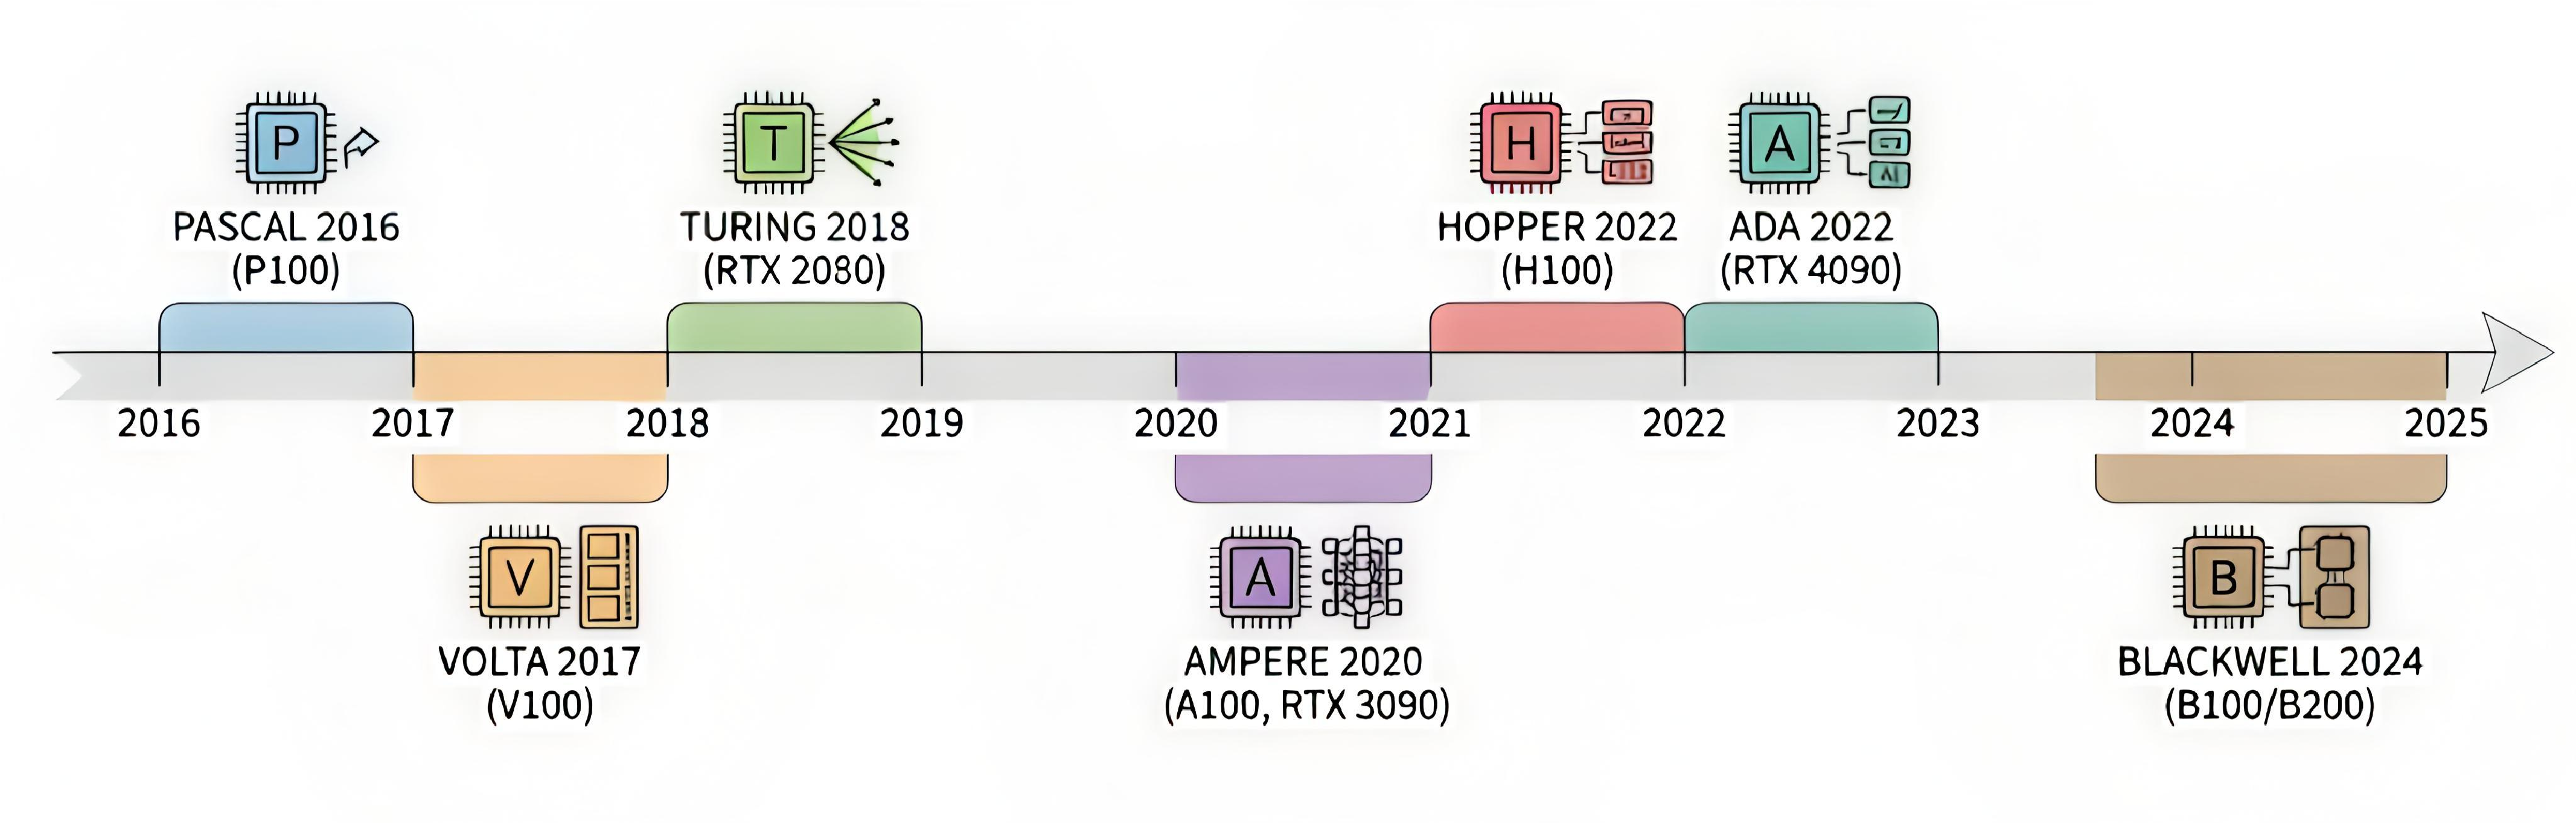
\includegraphics[width=\linewidth]{nvidia_gpu_evolution.pdf}
  \caption{NVIDIA GPU 架构与代表性产品演进}
  \label{fig:nvidia_gpu_evolution}
\end{figure}

在大多数高校、研究所与中小企业的实际环境中，受预算与采购周期限制，GPU 集群往往经历多次分批采购，而旧设备报废周期较长，集群中常同时包含多代 GPU（例如部分 A100 或 H100 与大量 RTX 3090/4090、甚至更早的 V100/RTX 2080），单机内也可能混用不同显存与互联配置，难以做到“全集群同构”，由此形成\emph{显存异构}与\emph{算力异构}并存的局面\cite{whale,hetpipe2020}。
然而，主流并行训练框架（如 Megatron-LM、DeepSpeed）在设计时多假设同构设备与统一拓扑\cite{megatron2021,zero2020}，在异构集群上直接使用容易出现以下问题：负载无法按算力与显存合理分配，低显存设备成为瓶颈而高端卡显存资源利用率低，以及计算最慢的节点拖慢整体迭代速度\cite{whale,hetpipe2020}。
对于单层计算与显存相对均匀的传统大语言模型，尚可通过“按层数或算力比例”划分在一定程度上缓解异构带来的影响。
而对于 MLLMs，其模块间在层类型、参数量与激活体积上的固有差异与设备能力差异相互叠加，使得简单的模型划分难以实现负载均衡。
因此，在显存与算力异构的 GPU 集群上高效训练 MLLMs，是学术界和工业界共同面临且亟待解决的问题。

从系统层面看，异构带来的问题不仅在于单卡能力差异，还在于拓扑与调度。
节点内 NVLink 与节点间 InfiniBand 的带宽可相差一个数量级以上，若流水线并行或张量并行的划分未考虑链路差异，跨节点通信极易成为瓶颈。
同时，MLLMs 各训练阶段对编码器、投影层与 LLM 基座的冻结策略不同，导致同一模型在不同训练阶段下各模块的计算与显存开销发生明显变化。
若沿用固定的模型划分与调度，难以在整轮训练中保持负载均衡。
即便划分与调度已得到优化，在异构流水级上采用全局统一的重计算配置仍难以同时满足各设备的显存约束。
因此，面向异构集群的 MLLMs 训练需要同时考虑硬件拓扑、模型结构、多训练阶段以及流水级差异化的显存—计算权衡，通过自适应的划分、高效的调度与按流水级配置的重计算策略协同提升训练效率。

综上所述，硬件层面的设备异构与模型层面的模块异构、分阶段冻结相互交织，使得异构集群上的 MLLMs 训练同时面临负载分配、算存资源利用、显存—计算权衡等多维约束，构成了当前有限资源下高效训练的核心难点。
随着云上与混合部署中弹性训练与按需资源供给的普及，集群内设备型号与拓扑将更加多样，这对异构感知的划分、调度与重计算配置提出了更高要求\cite{frenzy_memory2024,nvidia_training_guide,arnold2025}。
为此，本文基于 Megatron-LM 主流并行训练框架，针对 MLLMs 的模块结构异构与分阶段冻结特性，结合异构 GPU 集群中显存与算力的多维差异，研究细粒度的混合并行划分与重计算优化技术，旨在提出一套面向异构 GPU 环境的自适应并行训练方案，以提升异构 GPU 集群下 MLLMs 的训练效率。

\section{国内外研究现状与挑战}

本节从文献角度归纳与本文密切相关的研究脉络，先概述多模态大语言模型并行训练策略研究现状及其同构假设的局限，再综述面向异构 GPU 集群的并行训练工作，最后归纳重计算相关研究及其在异构 GPU 场景下的不足。

\subsection{多模态大语言模型并行训练策略研究现状}

Kaplan 等\cite{kaplan2020scaling} 通过系统实验提出扩展定律（Scaling Law），指出模型性能会随参数量与训练数据量的增加而提升；Chinchilla\cite{chinchilla2022} 进一步从计算最优角度表明参数规模与训练词元（token）数应近似同比例扩展，后续研究\cite{beyond_chinchilla2024} 又将该缩放规律拓展到推理成本约束下的最优配置。
基于上述研究，多模态大语言模型普遍沿着“更大参数规模+更大数据规模”的路径持续演进。

自 Transformer\cite{vaswani2017} 提出以来，语言模型规模呈持续扩张趋势，参数量由 BERT\cite{bert} 的亿级逐步发展到 GPT-2\cite{gpt2}、T5\cite{t5} 的十亿级，并进一步扩展至 GPT-3\cite{brown2020gpt3}、GPT-4\cite{openai2023} 以及 DeepSeek-V3\cite{deepseek2024}、Qwen2.5\cite{qwen2024} 等模型所代表的千亿级规模。
在此基础上，MLLMs 通过引入视觉编码器并与语言模型进行跨模态对齐，形成了以 BLIP-2\cite{blip2}、InstructBLIP\cite{instructblip2023}、LLaVA/LLaVA-1.5\cite{llava2023,llava15_2023}、Flamingo\cite{flamingo2022}、Qwen-VL\cite{qwenvl2023}、InternVL\cite{internvl2024} 和 MiniGPT-4\cite{minigpt4} 等为代表的技术谱系，其模型规模已覆盖数十亿至数千亿参数，训练数据规模也由百万级图文对扩展至十亿级样本（如 LAION-5B\cite{laion5b2022}）。
相关工作已从模型架构、跨模态对齐策略、数据构建与系统效率等维度对该领域进行了系统总结\cite{mllm_survey_acl2024,comprehensive_mllm_survey2024,mllm_datacentric2024}。
单卡或单机在显存容量和计算吞吐上已难以支撑完整训练流程\cite{megatron2021,megatron2020}，并行与分布式训练因此成为大模型与 MLLMs 训练的基础技术路径\cite{zero2020,zero2021}。

除了模型的参数规模，训练数据的规模同样持续扩大。图像方面，Open Images\cite{open_images}、COCO\cite{coco2014} 等海量图片数据集需 TB 级存储，LAION-5B 等开放图文对达数十亿样本。
文本方面，Common Crawl、The Pile\cite{pile2020} 等为 LLM 预训练提供数百 GB 至数万亿词元量级的语料。
视频方面，YouTube-8M\cite{youtube8m}、WebVid\cite{webvid2021} 等基准需 PB 级存储与高吞吐数据管线，多模态理解与推理则依赖 VQAv2\cite{vqav2}、TextVQA\cite{textvqa2019} 等数据集与长上下文基准\cite{long_context_benchmark2024}。
在单机无法存储完整数据集与模型的前提下，并行训练成为必然选择。

在并行策略方面，工业界与学术界在同构 GPU 集群上已形成以模型与数据切分为核心的多维混合并行，以及以状态分片为核心的 ZeRO 系列两大技术路线，并被 Megatron-LM、DeepSpeed 等并行训练框架广泛应用于千亿级参数 MLLMs 训练\cite{megatron2021,zero2020,zero2021}。
多维混合并行通过在不同维度上划分模型或数据以降低单卡负载：\emph{数据并行}\cite{pytorch_ddp,sergeev2018horovod} 在各设备组上复制完整模型、按批次划分样本，通信集中在梯度 AllReduce，实现简单且扩展性好；
\emph{张量并行}\cite{megatron2020,megatron2021} 将单层内矩阵按行或列切分到多卡，降低单卡显存，是千亿级稠密模型的主流选择；
\emph{流水线并行}将模型按层划分为若干流水级并分配到不同设备，有效支持超大规模模型的并行训练，但需借助更精细的调度以缓解流水线气泡、提高 GPU 利用率。
此外，\emph{序列并行}\cite{megatron2021}、\emph{专家并行}\cite{gshard} 等可与张量、流水线并行组合，以进一步扩展训练规模。
NVIDIA 的 Megatron-LM\cite{megatron2021,megatron2020} 联合使用张量、流水线与数据并行，已支撑在数千张同构 GPU 上训练千亿至万亿级参数的大语言模型。
零冗余优化器 ZeRO\cite{zero2020,zero2021} 在数据并行的基础上将优化器状态、梯度与参数分片存于各卡、按需聚合，显著降低单卡显存，但引入较多卡间通信；ZeRO-Infinity\cite{zero2021} 进一步将部分状态卸载至 CPU 或 NVMe；ZeRO++\cite{zeroplusplus} 则通过量化与通信优化削减跨节点开销。

% 在同构集群的自动并行方向，Galvatron\cite{galvatron2022} 针对 Transformer 将策略搜索与编译优化结合；Aceso\cite{aceso2024} 通过迭代瓶颈缓解联合优化通信与显存；UniAP\cite{uniap2025} 将层间与层内并行统一为混合整数二次规划以搜索全局配置；Colossal-Auto\cite{colossal_auto} 则将自动并行与重计算联合自动化。

% 上述方法多在\emph{同构}集群上为全部设备配置统一的重计算粒度与子模块集合。

然而，主流训练框架在设计时多假设\emph{同构} GPU 集群与相同 Transformer 层堆叠的语言模型，对 MLLMs 的\emph{模块异构}（编码器、投影层、LLM、生成器结构各异）与\emph{分阶段冻结训练}考虑不足。
以 Megatron-LM 为例，其在同构集群上训练 MLLMs 时，编码器与生成器的并行方式通常被动跟随 LLM 基座，缺乏面向各子模块算力与显存需求的细粒度映射，典型策略如图~\ref{fig:megatron_mllm} 所示\cite{disttrain2025}。
面向 MLLMs 的模块结构，DistMM\cite{distmm2024} 针对子模块差异组合张量并行与数据并行，DistTrain\cite{disttrain2025} 通过解耦模态编码器、LLM 基座与模态生成器的训练流程分别分配资源且配置并行策略，在同构集群上提高了训练 MLLMs 时集群的利用率。
在显存优化方面，Korthikanti 等\cite{megatron2023} 在 Megatron-LM 中提出序列并行与选择重计算，与张量并行协同以降低激活显存；Colossal-Auto\cite{colossal_auto}、Mist\cite{mist2025}、AdaPipe\cite{adapipe2024} 等工作进一步将重计算与自动并行或流水线划分联合搜索。

总体而言，上述面向 MLLMs 的并行训练方法多建立在同构 GPU 集群假设之上，忽视了异构设备间显存容量与计算吞吐的差异，对\emph{分阶段冻结训练}所引起的计算与显存负载的动态变化也缺乏针对性适配。
即便在同构集群中沿用上述策略，仍易诱发流水级负载失衡与局部显存瓶颈；在设备能力分布相对均衡而子模块算存需求差异显著的条件下，上述问题将进一步加剧。

\begin{figure}[htbp]
  \centering
  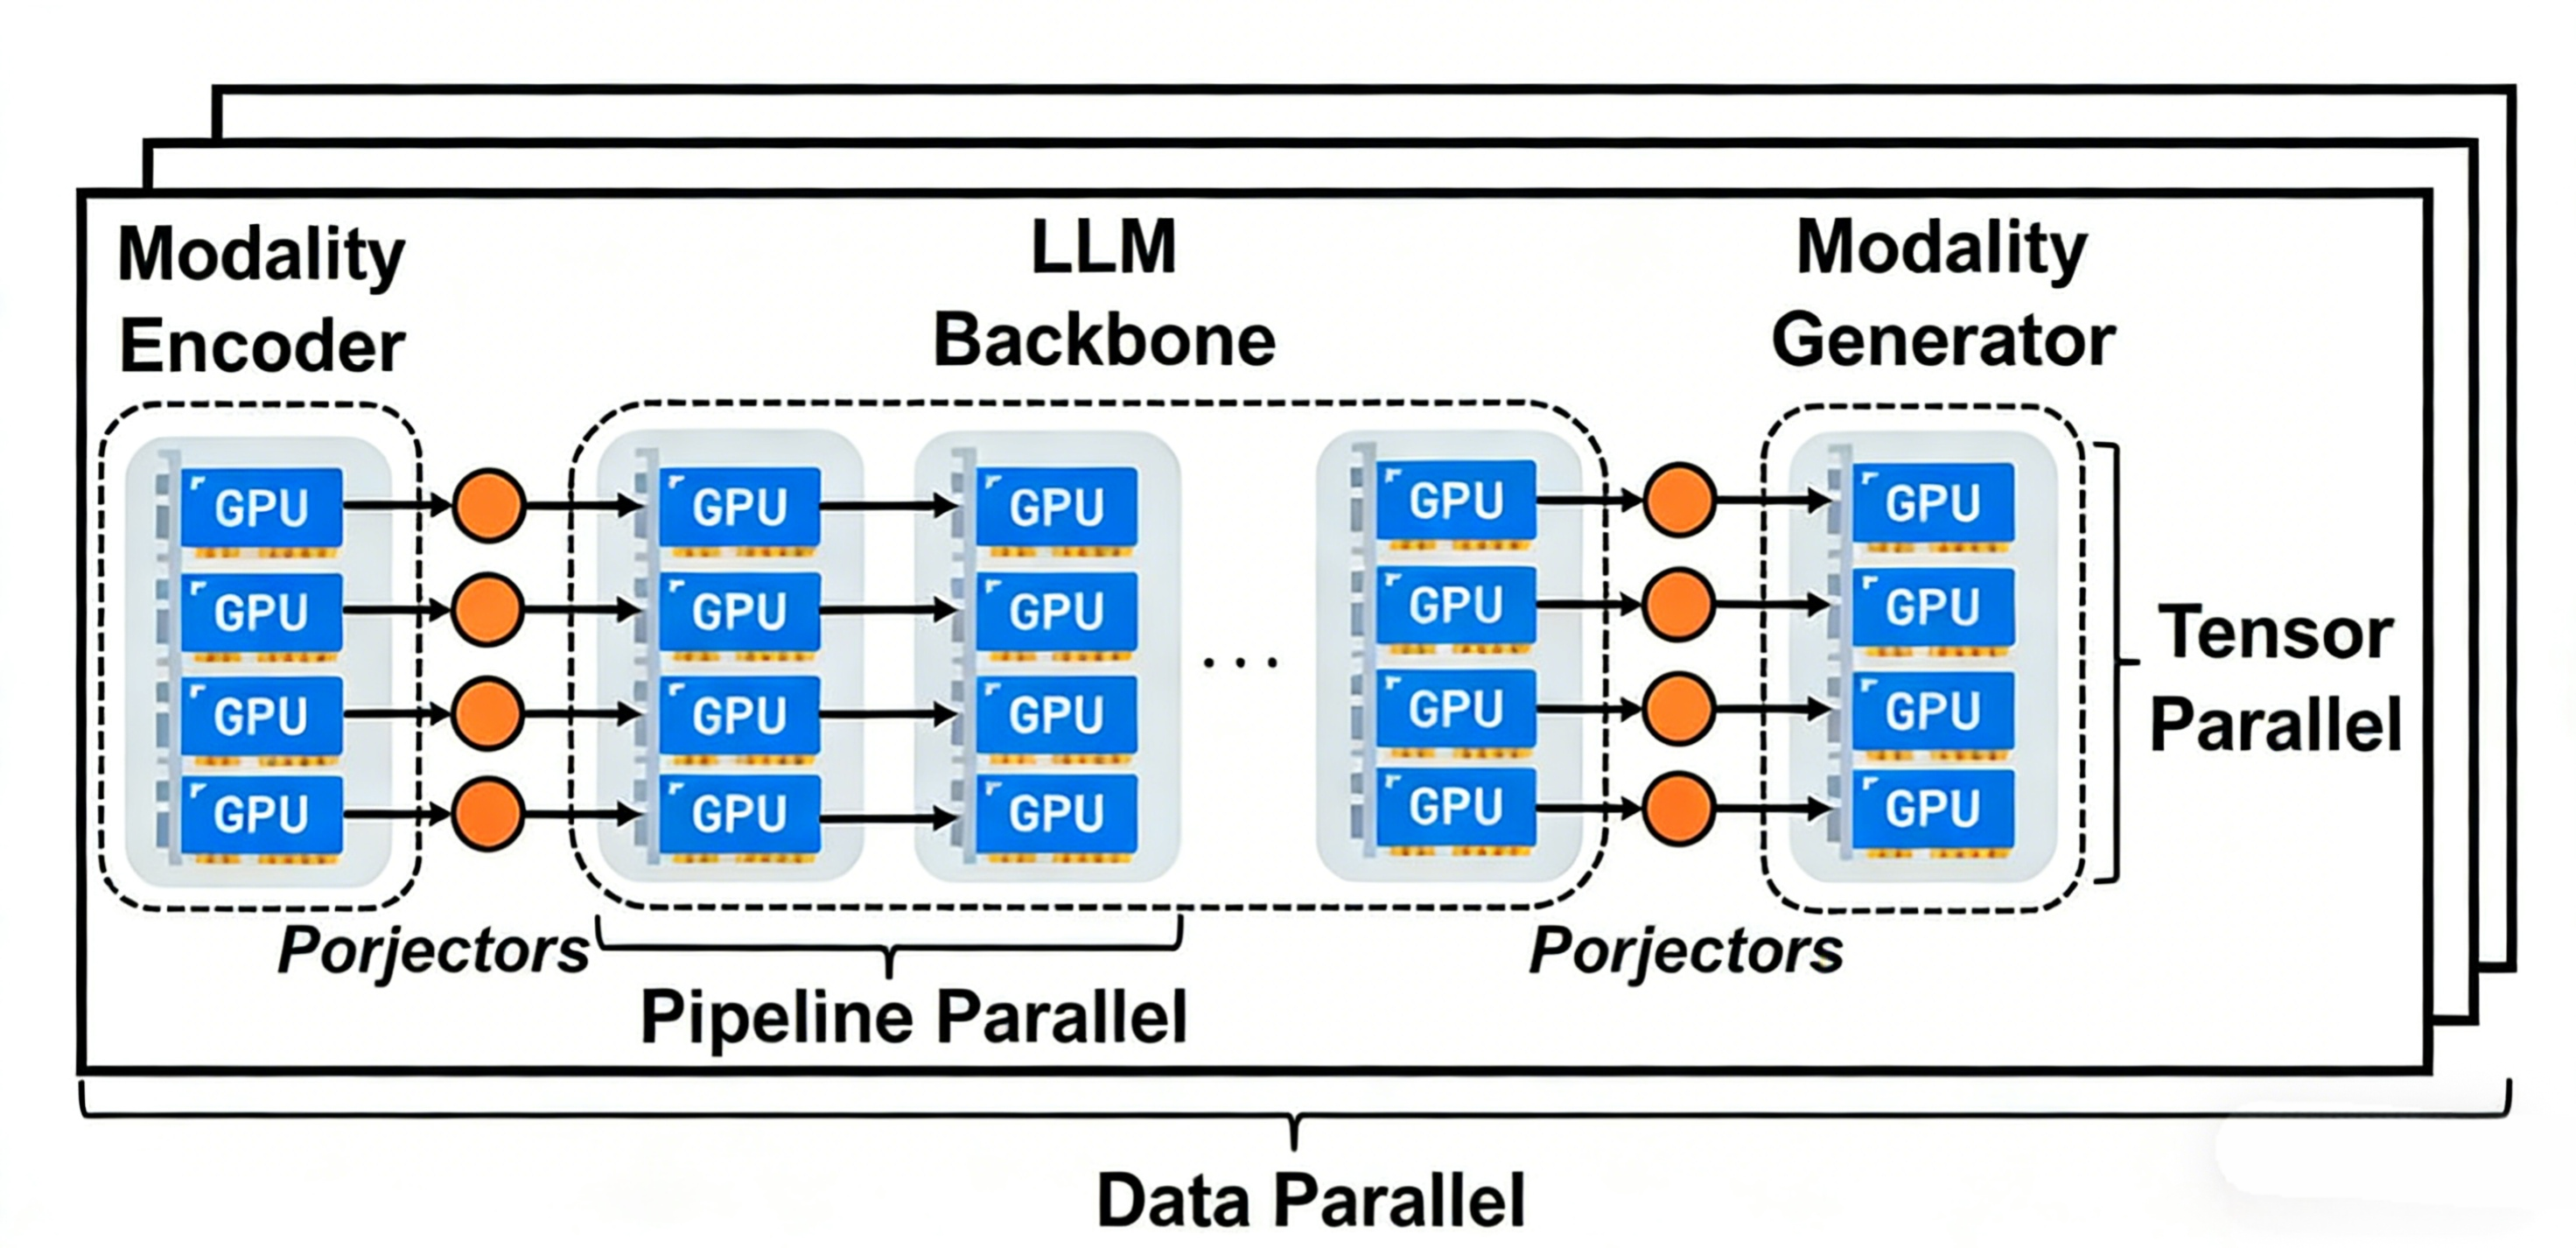
\includegraphics[width=\linewidth]{fig02_megatron_mllm.jpg}
  \caption{使用 Megatron-LM 框架在同构集群上训练多模态大语言模型的典型并行配置}
  \label{fig:megatron_mllm}
\end{figure}

\subsection{异构 GPU 集群并行训练策略研究现状}

受预算与采购周期限制，实际训练集群往往由多代、多型号 GPU 混合组成，呈现显著的显存与算力异构\cite{whale,hetpipe2020}。
将面向同构集群的并行技术与重计算策略直接用于异构 GPU 集群时，不同显存容量、算力与互联带宽的 GPU 设备会被视为同构的设备，低显存或低算力节点易成为整个系统的瓶颈，高端设备资源利用率不足，整体训练效率下降\cite{whale,hetpipe2020}。
针对上述问题，学术界已开展异构 GPU 感知的并行规划与资源调度研究。

早期工作如 HetPipe\cite{hetpipe2020} 将流水线并行与数据并行结合，借助虚拟工作节点（VW）在异构设备间分配负载，但未显式建模设备排列与通信拓扑，也未针对 MLLMs 的模块异构与分阶段冻结开展联合设计。
Whale\cite{whale} 从显存与算力差异出发进行硬件感知负载均衡，按异构 GPU 算力比例划分模型与数据批次，但其划分主要围绕设备算力展开，对模型模块异构带来的计算与显存差异覆盖仍不充分。
AMP\cite{amp2022} 在异构环境下自动搜索并行策略，综合考虑模型异构与设备异构，通过开销模型与动态规划得到近似最优配置；然而其划分粒度偏粗，通信与显存估计精度不足，难以支撑更细粒度的高效映射。

近年来，面向异构 GPU 集群的分布式训练系统在“异构感知并行规划—资源编排—代价建模”等方向上持续演进：HetHub\cite{hethub2024} 统一规划通信器、性能预测器与自动并行以适配多厂商 GPU；HexiScale\cite{hexiscale2024} 将多种并行划分形式化，并通过层次图划分在异构环境中分配计算；Espresso\cite{espresso2025} 联合优化异构资源供给与流水级放置；Metis\cite{metis2024} 以异构感知搜索实现快速自动并行规划；HAP\cite{hap2024} 将 SPMD 并行优化建模为程序合成问题，联合搜索张量分片与通信方式。
总体而言，上述异构感知工作多数仍偏向通用语言模型，且仅对\emph{设备异构}做单一维度优化，对于 MLLMs 特有的\emph{模块异构}、\emph{分阶段冻结}等特性则缺乏针对性调优。

在异构 GPU 集群上，面向同构集群的全局统一重计算配置适用性也进一步下降：显存不足的流水级若配置偏保守，仍可能因中间激活过大而 OOM，导致训练过程无法进行；显存充裕的流水级则可能被强制对齐同等强度的重计算，引入冗余前向计算并延长迭代时间。
在 MLLMs 模块异构与分阶段冻结并存的场景下，如何在与划分、调度协同的前提下按流水级差异化配置重计算，仍缺乏系统化研究。

除多维混合并行外，以 ZeRO 为代表的状态分片路线在异构 GPU 集群上训练 MLLMs 时亦面临局限：ZeRO\cite{zero2020,zero2021} 引入大量 All-Gather/All-Reduce 通信，在多节点集群中易成为瓶颈；MiCS\cite{mics2022} 难以结合设备算存差异与冻结阶段切换实现细粒度、动态的负载自适应；ZeRO++\cite{zeroplusplus} 的量化与通信优化可能带来精度与通用性代价；AMSP\cite{amsp} 等侧重跨节点通信削减，对集群内存储、算力与带宽的细粒度异构利用仍有限。
因此，在异构 GPU 集群上高效训练 MLLMs，仍需在 Megatron-LM、DeepSpeed 等现有框架基础上，引入对设备能力、模型模块结构与训练阶段的联合感知，实现划分、调度与重计算的协同自适应优化。

\subsection{研究问题与挑战}

围绕异构 GPU 集群上的多模态大语言模型训练，本文聚焦的核心研究问题是：在设备显存、算力与带宽不一致的真实异构 GPU 集群环境下，如何针对 MLLMs 的模块异构结构与分阶段冻结训练的特性，联合优化模型划分、流水线调度与重计算配置，在满足显存约束与收敛正确性的前提下最小化迭代时间，提升端到端训练速度。

为回答这一问题，本文面临以下三项关键挑战。
第一，模块异构与设备异构耦合导致负载失衡。MLLMs 由编码器、投影层与 LLM Backbone 等多个模块构成，不同模块在计算量与显存占用上差异显著。
当其与异构 GPU 的算存能力差异叠加时，传统按层均分或按单一硬件指标划分模型的方法容易形成瓶颈流水级，导致整体吞吐受限。
第二，冻结阶段切换使最优并行策略动态变化。
在不同冻结策略中，可训练参数集合动态变化，反向计算与梯度同步开销随之动态变化，静态划分与固定调度难以在全流程保持高效。
第三，统一的重计算策略难以兼顾显存安全与训练效率。在使用更大批次与更长序列训练时，部分流水级存在显存瓶颈并可能发生 OOM。

基于上述挑战，本文的研究目标是构建一套面向异构 GPU 集群上多模态大语言模型训练的联合优化框架：在模型划分层面考虑异构 GPU 设备与冻结导致的模型算存需求的变化，在调度层面利用冻结信息剪枝冗余反向与通信，在重计算策略层面按流水级配置差异化重计算策略，从而形成“划分—调度—重计算”多级优化框架。
具体而言，挑战一主要对应框架的划分层，侧重模块异构与设备异构耦合下的负载均衡；挑战二则要求划分与调度随冻结状态协同调整，并消除冻结场景下的冗余反向与通信，对应框架的划分层与调度层，由第三章 MMoH 的并行策略规划器与提前终止调度器共同解决；挑战三主要对应框架的重计算层，由第四章 HR-MMoH 在 MMoH 基础之上按流水级进行差异化重计算配置，以支撑更大批次与更长序列训练并进一步压缩迭代时间。

\section{研究内容与贡献}

围绕异构 GPU 集群上多模态大语言模型的高效训练这一总体目标，本文将研究工作分解为两个层次递进、相互衔接的子问题。
第一，划分与调度子问题：在设备显存与算力异构、且训练过程伴随分阶段冻结切换的条件下，如何自动生成面向多模态大语言模型的细粒度模型划分、设备映射与流水线调度方案，使各流水级计算负载与异构设备能力相匹配；如何随各训练阶段的冻结状态生成相应的划分与映射配置，并在流水线执行中剪枝连续冻结流水级的冗余反向计算与级间通信，以提升 GPU 利用率与训练吞吐。
第二，重计算子问题：在第一子问题所确定的并行执行骨架（设备拓扑、模型划分与冻结感知调度）之上，当训练规模向更大批次与更长序列扩展时，如何按流水级配置差异化的重计算策略，在各设备显存约束下尽可能降低重计算引入的额外计算开销，进一步缩短迭代时间。

针对上述两个子问题，本文依次提出 MMoH 与 HR-MMoH 两种方法，分别针对划分—调度与重计算两个层次的优化任务，研究内容与贡献如下。

\subsection{MMoH：多模态大语言模型在异构 GPU 集群上的混合并行方法}

针对异构 GPU 环境中显存与算力差异导致的设备利用率低、模块结构差异引发的模型划分困难，以及分阶段冻结训练造成的计算与显存需求动态变化等问题，本文提出一种面向异构 GPU 集群的多模态大语言模型混合并行训练方法。该方法通过为不同计算设备分配不同规模的模型分片，实现对计算资源与显存空间的协同利用，从而提升训练吞吐并缩短迭代时间。进一步地，为适应多阶段冻结训练过程，该方法能够感知各阶段冻结状态并与并行划分方案协同调整，同时在连续冻结的流水级上省略不必要的反向计算与级间通信，在保证模型收敛性的前提下进一步提升异构设备的有效利用率与整体训练效率。
MMoH 承担本文两级方法中的划分与调度层，其输出包括设备拓扑、模型映射及冻结感知的流水线调度策略，构成后续重计算优化的优化对象与约束条件。

\subsection{HR-MMoH：多模态大语言模型在异构 GPU 集群上的重计算方法}

针对现有重计算策略多采用全局统一配置、未考虑异构 GPU 集群中设备显存与算力差异的问题，本文提出一种面向异构设备与多模态大语言模型的重计算优化方法。
HR-MMoH 以 MMoH 的划分与调度结果为输入，将重计算决策粒度由全局统一下沉至流水级差异化：以各设备显存上限为约束，对显存受限流水级采用较强的重计算以降低激活驻留，对显存充裕流水级则减少冗余重算，从而在满足显存约束的前提下最小化重计算引入的额外计算开销。
HR-MMoH 不改变 MMoH 的划分与调度策略，而是在其基础之上与之共同构成“划分—调度—重计算”多级优化链路，进一步提升异构 GPU 集群上 MLLMs 的端到端训练效率。


\section{论文组织结构}

本文共分为以下五个章节，具体结构如下：

第一章为绪论。首先从多模态大语言模型的训练需求与异构 GPU 集群的现状两个方面阐述研究背景与意义，随后分别从多模态大语言模型并行训练和异构 GPU 集群并行训练两个维度梳理国内外研究现状，最后介绍本文的研究内容与主要贡献。

第二章为相关工作。首先介绍多模态大语言模型的模型架构、训练过程以及数据并行、模型并行与 ZeRO 等主流并行训练技术，其次综述异构 GPU 集群上的并行训练策略与工业实践，最后阐述重计算技术的基本原理、分类及主流实现的局限性。

第三章介绍多模态大语言模型在异构 GPU 集群上的高效混合并行技术 MMoH，重点阐述需求驱动的设备拓扑识别、复合粒度模型抽象、冻结感知划分及提前终止流水线调度方法，并给出实验评估。

第四章介绍多模态大语言模型在异构 GPU 集群上的重计算技术 HR-MMoH，详细说明如何在异构 GPU 集群与不同模型模块间实现重计算策略的细粒度自适应配置并进行实验验证。

第五章为总结与展望。概括本文主要创新点，归纳本文的研究局限，并对后续研究问题与思路作简要展望。

\chapter{相关工作}

本章从多模态大语言模型、并行与分布式训练基础、异构 GPU 集群并行训练策略以及
梯度检查点优化等方面对国内外相关研究进行综述。
如今，基于 Transformer 的大语言模型在包括自然语言处理\cite{brown2020gpt3,openai2023}、
图像识别\cite{vit2020}、多模态\cite{clip2021}、图学习与推荐系统等众多前沿领域和
下游任务上大放异彩。
然而，随着模型参数的增加和数据规模的扩大，模型结构越来越复杂、
模型参数量越来越大、训练数据越来越多，
导致单个设备已经无法完成模型和数据的存储，
多模态大语言模型的训练越来越有难度。
为了解决上述问题，目前学界已经提出并应用了多种并行策略来实现和优化大模型的训练。
然而，目前传统的并行策略往往忽略了并行训练平台的异构性，
由于服务器集群中常常存在多种型号的 GPU 和网络连接，
导致集群中存在着存储异构、算力异构和网络异构。
在这样的复杂集群环境下，
传统的并行策略会因为缺乏对异构环境的感知和适应而导致性能表现急剧下滑。
因此，下文将主要从现有大模型的并行训练策略出发，
对并行训练的研究现状进行详细论述，并讨论各个并行策略在异构环境下的优缺点。

\section{多模态大语言模型}

\subsection{多模态大语言模型架构}

多模态大语言模型（MLLMs）通常由 Modality Encoder、Input Projector、LLM Backbone、
Output Projector 等模块组成。
Modality Encoder 负责将不同模态的输入数据（如图像、视频、音频）编码为模型可理解的表示，
常采用预训练的视觉模型如 CLIP\cite{clip2021}、ViT\cite{vit2020} 等。
LLM Backbone 是模型的核心，通常为参数量巨大的 Transformer 基座模型（如 GPT 系列%
\cite{brown2020gpt3,gpt2}、LLaMA\cite{llama3}、T5\cite{t5} 等），
占据整个模型约 80\%--90\% 的参数量。
Modality Generator 一般为 Diffusion 类生成模型（如 Stable Diffusion\cite{stable_diffusion}），
根据 LLM 的输出生成图像、视频等其它模态数据。
前后两个 Projector 用于将不同模态映射到共享语义空间，
可能是 Linear 层、Transformer 层或 Q-Former\cite{blip2} 等结构。
Blip-2\cite{blip2} 率先提出冻结预训练 Encoder 与 LLM、仅训练轻量 Projector 的范式，
后续 NextGPT\cite{nextgpt}、DreamLLM\cite{dreamllm} 等工作均沿用并发展了此类架构。
多模态大语言模型的这种模块异构性使得不同层在算力、显存和通信上的需求差异很大，
在异构 GPU 集群上部署时面临独特的挑战。

\subsection{多模态大语言模型训练数据}

为获得满意的性能，大语言模型与多模态大语言模型通常依赖大规模数据训练。
例如图像数据集 JFT-3B 包含约 30 亿张图片，
Common Crawl 网页数据包含数千亿 tokens，
Open Image\cite{open_images} 需约 18TB 存储，
YouTube-8M\cite{youtube8m} 等视频数据集甚至需要 PB 级存储。
在单个硬件加速器上既无法存储完整模型参数，也无法容纳如此大规模的训练数据，
因此并行训练（数据并行、模型并行及其组合）成为必然选择。
数据规模与模型规模的持续增长，
也使得对并行策略的通信效率、存储划分和异构适应性提出了更高要求。

\subsection{多模态大语言模型训练目标}

多模态大语言模型的训练通常分为多个阶段，如模态对齐、指令微调等，
不同阶段会冻结不同模块（如冻结 LLM 仅训练 Projector，
或冻结 Encoder 与 LLM 仅训练部分层）。
冻结会显著改变各模块的反向计算量与显存占用（如优化器状态仅需为未冻结参数维护），
并影响流水线中各 stage 的负载均衡。
在异构 GPU 集群下，这种因阶段和冻结策略带来的“模型异构”与设备异构叠加，
进一步增加了并行策略设计与自动调优的难度。

\section{并行与分布式训练基础}

\subsection{常见并行策略}

数据并行（Data Parallelism）被广泛用于处理数据规模过大的情况，
其核心思想是通过将训练数据在所有计算设备上划分，
而每个计算设备都持有一份完整的模型参数\cite{parameter_server,horovod,pytorch_ddp}。
如图\ref{fig:data_parallel}所示，在训练过程的每次迭代中，
每个设备可以独立地使用本地模型参数和批次数据计算对应批次的梯度；
然后，所有设备在下一次迭代之前进行通信操作，
将各自计算得到的梯度数据进行同步，
从而保证模型参数的一致性和结果的正确性。
数据并行训练因其隐式性和直观性而成为并行训练最早提出的策略，
也是实际应用中最常见的方式。
PyTorch 框架中提供了 DistributedDataParallel\cite{pytorch_ddp} 工具用于数据并行训练。
Horovod\cite{horovod} 将数据并行策略适配到了多个框架中。
Parallax\cite{parallax} 则根据模型的特点灵活地使用参数服务器（Parameter Server）或
All-Reduce 通信原语进行数据同步，优化了数据并行中的通信开销。
然而，数据并行存在着明显限制：每个 GPU 都保存模型权重的完整副本，
因此不能直接用于训练具有大量参数的模型，限制了模型规模的扩展；
同时，数据并行也将模型训练的工作限制在了单个计算设备内，
无法通过设备并行的方式加速训练过程。

\begin{figure}[htbp]
  \centering
  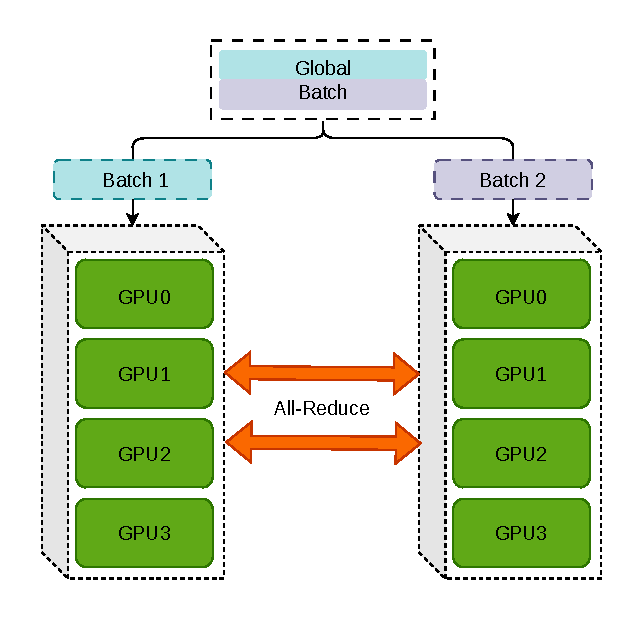
\includegraphics[width=0.75\linewidth]{fig03_data_parallel}
  \caption{数据并行}
  \label{fig:data_parallel}
\end{figure}

模型并行（Model Parallelism）是实现大模型训练的有效途径，
包括张量并行（Tensor Parallelism）\cite{megatron2020} 和
流水线并行（Pipeline Parallelism）\cite{gpipe}。
张量并行的核心思想是将模型在层内进行划分，
每个计算设备分别持有模型一部分的层内张量，它们组合在一起是一份完整的张量，
从而将模型的参数和计算任务分别绑定到不同的相互连接的设备上。
如图\ref{fig:tensor_parallel}所示，在训练过程的每次迭代中，
每个计算设备只负责模型一部分参数的计算，
然后通过中间激活值和梯度值的通信，使模型可以进行下一层的计算。
Megatron-LM\cite{megatron2020} 提出了针对 Transformer 模型张量并行的训练方法，
对每两个连续层的权重首先按行（输入维度）划分，再按列（输出维度）划分，
消除了同步第一层中间输出的需要，但随后仍然需要大量的跨设备通信。
GShard\cite{gshard} 提出了在计算图层面进行张量并行优化的思路。
然而，目前的张量并行方式受限于 GPU 服务器集群中的带宽情况，尤其是跨节点带宽，
其并行规模无法进行大规模扩展，往往需要结合其他并行方式一起加速。

\begin{figure}[htbp]
  \centering
  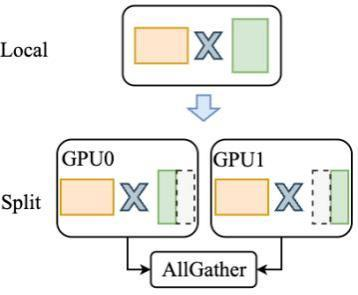
\includegraphics[width=0.75\linewidth]{fig04_tensor_parallel}
  \caption{张量并行}
  \label{fig:tensor_parallel}
\end{figure}

流水线并行的核心思想是将模型在层间进行划分，
每个计算设备分别持有整个模型的若干层，称为一个 stage；
这些 stage 组合起来是一份完整的模型。
如果直接将不同设备上的 stage 串行地进行训练，
则会导致每个 stage 训练过程中只有一个设备在进行计算，设备利用率极低。
如图\ref{fig:pipeline_parallel}所示，流水线并行针对训练数据进一步划分为多个
micro-batch，依次输入到模型中进行计算。
尽管各级流水线在不同的 micro-batch 之间存在数据依赖，
然而 batch 之间数据是相互独立的，
从而每个 micro-batch 可以依次进行模型训练，实现流水线的训练过程，
大大减少计算设备的空闲时间。
GPipe\cite{gpipe} 提出了使用 micro-batch 的流水线并行方式，
通过设计多级流水减少了 Bubble 的空闲。
PipeDream\cite{pipedream2019} 提出了 1F1B（1 次前向 1 次反向），
通过异步调度的方式进一步减少了 Bubble 的空闲。
TeraPipe\cite{terapipe} 则在自回归模型的单个训练 sequence 中使用 token 级流水线并行，
实现了更细粒度的流水线并行。
数据并行、张量并行和流水线并行策略相互正交，可以一起用于并行训练。
由于流水线并行的通信量一般较小，且跨节点通信明显慢于节点内通信，
因此张量并行往往仅限于节点内训练，而流水线并行则用于跨节点训练，
以更好地利用硬件带宽\cite{megatron2020}。

\begin{figure}[htbp]
  \centering
  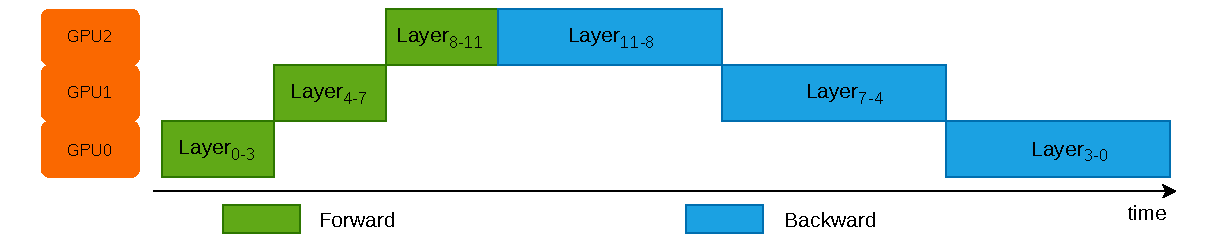
\includegraphics[width=0.8\linewidth]{fig05_pipeline_parallel}
  \caption{流水线并行}
  \label{fig:pipeline_parallel}
\end{figure}

\subsection{多维混合并行}

ZeRO\cite{zero2020} 是微软 DeepSpeed 团队提出的零冗余优化器技术，
针对大规模深度神经网络中数据并行训练进行高效优化。
如图\ref{fig:zero}所示，在模型训练中，
各部分的存储占用从高到低依次为优化器状态、梯度和参数。
ZeRO 通过将以上三部分分别划分到每个计算设备中，
进而减少存储开销和提高 GPU 利用率来扩展大语言模型的训练。
在训练过程中，ZeRO 通过前向和反向的多次通信同步数据，保证训练结果的一致性。
目前，学界已经提出了一些针对 ZeRO 的通信方面的改进工作。
MiCS\cite{mics2022} 是在云服务环境下针对 ZeRO 的通信数据量进行减少和优化；
ZeRO++\cite{zeroplusplus} 基于量化技术减少 ZeRO 的通信数据量；
AMSP\cite{amsp} 则将 ZeRO 的划分方式扩展到一个统一划分空间，
寻找通信开销最小的策略，进一步扩展了大模型训练的规模。

\begin{figure}[htbp]
  \centering
  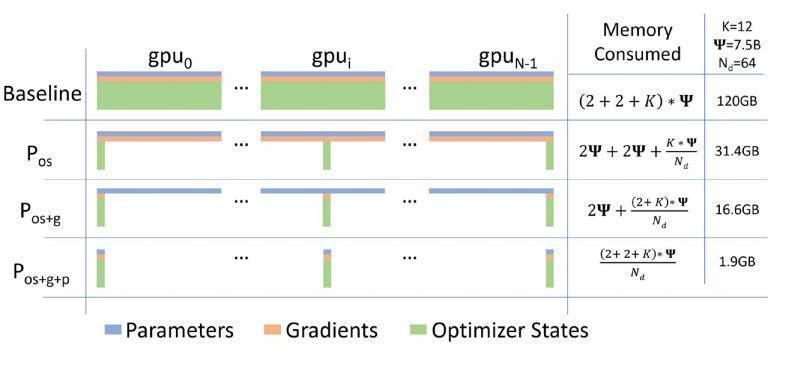
\includegraphics[width=0.8\linewidth]{fig06_zero}
  \caption{零冗余优化器 ZeRO}
  \label{fig:zero}
\end{figure}

\section{异构 GPU 集群并行训练策略}

在存储方面，由于不同 GPU 之间的存储不一致，
传统的并行策略会导致存储负载不均衡，
大存储的设备会出现存储利用不充分的问题，影响了模型训练的扩展性。
在算力方面，由于不同 GPU 之间的算力不一致，
传统并行策略会导致“木桶效应”，不仅使得计算资源利用率下降，
还导致整体训练速度的降低。
在网络方面，由于集群中存在的不对称的多级网络连接，
使得不同设备之间的通信开销相去甚远，
低带宽网络对应的通信将成为训练的性能瓶颈。
因此，面向异构 GPU 集群的并行训练策略成为近年来的研究热点。

HetPipe\cite{hetpipe2020} 结合了流水线并行（PMP）和数据并行（DP），
多个 GPU 被分组为虚拟工作节点（VW），以流水线方式处理小批量数据，
然后这些虚拟工作节点再通过数据并行提高训练的可扩展性和性能。
但是 HetPipe 没有考虑虚拟工作节点内部的异构设备排列方式，
对于通信开销和显存开销的考虑过于直观，而且完全没有考虑模型异构，
在如今的多模态大语言模型训练时不适用。

Whale\cite{whale} 是阿里巴巴团队提出的一种面向异构存储的 GPU 集群的并行训练优化方法。
由于实际 GPU 集群中存在的存储异构和算力异构问题，
Whale 提出了一种基于硬件感知的负载均衡算法，
通过按比例分配的方式为每个设备分配不同大小的批次数据和模型部分，
实现了数据并行与张量并行的负载均衡。
然而，Whale 没有考虑集群中普遍存在的网络异构性，
对于存储异构和算力异构的优化方法过于直观和简单，
并且是在子图的粗粒度下进行的划分和编译，也没有考虑 ZeRO 的并行方法，
因此仍然需要进一步的优化。

AMP\cite{amp2022} 是卡耐基梅隆大学团队提出的一种针对异构环境下大模型的
并行训练优化方法。
AMP 同时考虑了模型异构和设备异构，
针对模型中不同层的结构不同的情况进行了抽象和建模，
而针对集群中不同 GPU 存储异构和网络异构进行了近似计算。
在此基础上，AMP 基于 3D 并行方法（DP+TP+PP），
设计了一个详细的开销模型（Cost Model）以评估异构模型在异构环境下的计算和通信开销，
并通过动态规划算法确定最优的并行策略。
尽管 AMP 在传统的 3D 并行策略的基础上提升了异构环境下的性能表现，
但是 AMP 的并行维度是基于全局的粗粒度划分，开销模型的准确性不足，
并且没有考虑显存开销，
在实际的应用中会大概率发生内存不足（Out of Memory）的问题，
故而仍然具有很大的改进空间。

而与 ZeRO 相关的工作中，不论是 ZeRO、MiCS 还是 ZeRO++ 和 AMSP，
在面向大语言模型并行训练的异构性环境下，均存在着潜在的问题和提升的空间。
ZeRO 中存在着庞大的通信开销；
MiCS 中存在着对模型规模的限制，并且对于异构的网络连接中的高带宽连接利用率低；
ZeRO++ 的量化方法引入了潜在的信息损失和模型性能的下降，存在通用性问题；
AMSP 针对通信的优化思路同样局限于减少跨节点的通信量，
无法充分适应和利用异构集群中存在的不同存储、算力和网络带宽。

\section{梯度检查点优化}

在大规模模型与长序列训练中，为节省显存，
常采用梯度检查点（Gradient Checkpointing）技术，
即不保存所有层的中间激活，仅在部分层保存，
反向传播时对未保存的层进行重新前向计算以得到梯度。
全部重计算策略不保存任何中间激活，仅在需要时按需重算，
显存占用最低但计算量增加明显。
选择重计算策略则选择部分层作为检查点保存激活，在显存与计算之间取得折中。
细粒度重计算进一步在算子或更小粒度上决定保存与重算，
可结合模型结构和异构设备的显存与算力进行更精细的优化。
在异构 GPU 集群上，不同设备显存与算力差异大，
将梯度检查点与流水线划分、stage 分配结合，
可避免显存溢出并提高整体吞吐，是本文后续优化方向之一。
Colossal-Auto\cite{colossal_auto} 等工作对自动并行与激活检查点进行了统一自动化，
为面向异构环境的联合优化提供了参考。

\chapter{基于锐度比策略的自适应锐度正则化算法 SAMAR}

\section{引言}
% 正文内容

\section{SAMAR 算法设计与实现}

\subsection{锐度比策略设计}
% 正文内容

\subsection{算法实现}
% 正文内容

\section{SAMAR 算法的理论属性}

\subsection{基本假设}
% 正文内容

\subsection{收敛性分析}
% 正文内容

\section{实验验证}

\subsection{图像分类实验}
% 正文内容

\subsection{Hessian Spectrum 分析}
% 正文内容

\subsection{损失曲面可视化}
% 正文内容

\section{本章小结}
% 正文内容

\chapter{HR-MMoH: 多模态大语言模型在异构 GPU 集群上的重计算策略}

第二章分析了多模态大语言模型（MLLMs）在模块异构与分阶段冻结训练下呈现的计算与显存需求差异，第三章在此基础上通过 MMoH 框架解决了异构集群上的划分与调度问题。
在此背景下，本章进一步聚焦显存维度的瓶颈，提出 HR-MMoH（Heterogeneous Recomputation for training multimodal large language models on heterogeneous GPU clusters），
以异构感知的重计算策略补充第三章的工作。

\section{引言}
\label{sec:HR-MMoH-intro}

第三章介绍的 MMoH 框架通过需求驱动的设备拓扑、复合粒度划分与提前终止流水线调度，在异构 GPU 集群上显著提升了训练 MLLMs 的吞吐量。
然而，由于异构 GPU 集群中设备间显存与算力差异显著，在显存受限的节点上，仅靠流水线模型划分仍可能无法容纳较大批量的数据或者较长的序列输入，训练过程仍面临显存瓶颈。
\emph{重计算}（Recomputation）又称\emph{梯度检查点}（Gradient Checkpointing）\cite{chen2016checkpoint}，
通过在前向传播时少存部分中间激活值或者不存任何中间激活值、在反向传播时重新进行一次前向传播，把在前向传播时丢弃的中间激活值重新计算出来，
以算力换显存，在保持数学等价性的前提下支持更大批量、更长序列或更大参数的模型训练，是目前学术界和工业界广泛采用的缓解显存压力的技术。

现有主流框架（如 Megatron-LM）中的重计算策略多面向\emph{同构}集群设计：在同一训练任务中，
对所有流水级或所有设备采用统一的\emph{重计算粒度}（如整层重计算 Full Recomputation、子模块级重计算 Selective Recomputation）
与统一的\emph{层级划分方式}（如均匀分块 uniform、仅前若干层做检查点 block），
或对全体层采用相同的\emph{重计算子模块集合}（如仅 core\_attn、或 core\_attn+mlp+layernorm）。

然而，在异构集群上，各设备显存与算力差异显著：若在显存紧张的设备上采用过粗的重计算粒度或过少的重计算模块，
仍易发生 OOM，导致训练无法进行；
若在显存充裕的设备上采用过细的粒度或过多的重计算子模块，则会带来不必要的重计算开销，
延长迭代时间并造成算力浪费。
因此，\emph{为了同构集群设计的的检查点策略难以在异构环境下同时兼顾显存利用率与计算效率}。

针对上述问题，本章介绍 HR-MMoH：
在 MMoH 的异构流水线划分与调度基础上，面向\emph{异构设备}的显存与算力差异，
设计\emph{异构感知的重计算}策略，使各流水级或各设备可根据自身显存与算力条件
采用差异化的重计算粒度与子模块重计算选择，在降低 OOM 风险的同时尽量减少多余重计算、平衡各流水级计算负载，
从而与第三章的划分与调度形成“划分—调度—显存优化”的联合优化。
\ref{sec:HR-MMoH-method}节形式化描述异构重计算策略的设计与实现思路，
\ref{sec:HR-MMoH-exp}节给出实验设置、结果与分析，\ref{sec:HR-MMoH-summary}节总结本章内容。

\section{异构重计算}
\label{sec:HR-MMoH-method}

\subsection{现有的重计算策略与定量分析}
\label{sec:megatron-recompute}

作为当前大模型分布式训练的主流框架，NVIDIA 推出的 Megatron-LM\cite{megatron2020,megatron2021,megatron2023} 大模型并行训练框架集中定义了与重计算相关的配置，
开发者通过命令行参数传入重计算配置，例如 \texttt{--recompute-granularity}、\texttt{--recompute-method}、\allowbreak \texttt{--recompute-num-layers}、\texttt{--recompute-modules}。

配置参数方面，表~\ref{tab:chap4-megatron-params} 给出 Megatron 中与重计算相关的主要参数及其含义。
其中 \texttt{recompute\_granularity} 决定整层（full）或子模块级（selective）重计算；
full 时须同时指定 \texttt{recompute\_method} 与 \texttt{recompute\_num\_layers}，selective 时二者须为 \texttt{None}，仅由 \texttt{recompute\_modules} 指定要重算的子模块。
\texttt{distribute\_saved\_activations} 为 \texttt{True} 时，可将 checkpoint 保存的激活在张量并行组内分片存储以进一步省显存，但仅对 full 粒度且未启用序列并行的情形有效。

\begin{table}[htbp]
	\centering
	\caption{Megatron-LM 重计算相关配置参数}
	\label{tab:chap4-megatron-params}
	\begin{tabular}{@{}p{3.5cm}p{2.8cm}p{\dimexpr\textwidth-3.5cm-2.8cm-4\tabcolsep\relax}@{}}
		\toprule
		参数 & 类型/取值 & 说明 \\
		\midrule
		\texttt{recompute\_}\\\texttt{granularity} & \texttt{None} $\mid$ \texttt{full} $\mid$ \texttt{selective} & 重计算粒度。\texttt{None} 表示不重计算；\texttt{full} 对整层做重计算；\texttt{selective} 仅对 \texttt{recompute\_modules} 中列出的子模块重算。 \\
		\texttt{recompute\_method} & \texttt{None} $\mid$ \texttt{uniform} $\mid$ \texttt{block} & 仅用于 \textbf{full} 粒度：如何划分“哪些层”做 checkpoint。\texttt{uniform} 为均匀分块，\texttt{block} 为仅对每流水级前若干层做 checkpoint。\textbf{selective 时必须为 None}。 \\
		\texttt{recompute\_num\_}\\\texttt{layers} & \texttt{None} $\mid$ 正整数 & 仅用于 \textbf{full} 粒度。\texttt{uniform} 时表示每个 chunk 的层数；\texttt{block} 时表示每个 stage 内做重计算的层数。\textbf{selective 时必须为 None}。 \\
		\texttt{distribute\_saved\_}\\\texttt{activations} & 布尔 & 为 \texttt{True} 时，将 checkpoint 保存的激活在张量并行组内分片存储；仅 \textbf{full} 粒度且非序列并行时有效。 \\
		\texttt{recompute\_modules} & 字符串列表 & 仅用于 \textbf{selective}。要重算的子模块名列表（见下文）。默认 \texttt{["core\_attn"]}。 \\
		\bottomrule
	\end{tabular}
\end{table}

\textbf{整层重计算（full）}：以 Transformer 层为统一粒度做检查点；前向只保存每个“块”的输入，反向时重新执行该段前向再反传。
在 full 粒度下，\texttt{recompute\_method} 与 \texttt{recompute\_num\_layers} 共同决定流水级上多少个模型层只需要保存一个中间激活值。
\texttt{recompute\_method} 具体可以取一下以下两种值：
\begin{itemize}
	\item \textbf{uniform}（均匀分块）：将当前流水级内的所有层均匀分成多个 chunk，每个 chunk 包含 \texttt{recompute\_num\_layers} 层；
  每个 chunk 的输入被 checkpoint，chunk 内前向一次执行，反向时整个 chunk 先重计算再反传。
  chunk 数少则显存更省，但单次重算层数较多。
	\item \textbf{block}（仅前 N 层）：在当前流水级内，只对前 \texttt{recompute\_num\_layers} 层逐层做重计算；后续层不需要做重计算，正常存储中间激活。
  在显存允许时可减少重计算量，更充分利用显存。
\end{itemize}

\textbf{选择重计算（selective）}：在每一层内仅对 \texttt{recompute\_modules} 中列出的子模块做重计算，其余部分正常存激活。
此时 \texttt{recompute\_method} 与 \texttt{recompute\_num\_layers} 均须为设置为 \texttt{None}，且 selective 始终作用于所有流水级上的所有模型层。
模型每个子模块在各自的前向传播中根据用户指定的配置项\texttt{recompute\_modules} 决定舍弃哪些子模块的中间激活值，在反向传播时哪些模块的激活值需要重新计算。

选择性子模块方面，\texttt{recompute\_modules} 指定在 selective 粒度下要对哪些子模块做重计算。
不同子模块采用的重计算机制不同：标准 checkpoint 保存输入、反向时重新前向再反传；
Output-discarding checkpoint 在前向完成后丢弃该子模块输出的显存，在反向时通过梯度钩子函数再算一遍并写回，可进一步节省显存。
若未指定 \texttt{recompute\_modules}，则默认为 \texttt{["core\_attn"]}。
稠密模型下常用的“最省显存”组合为 \texttt{[core\_attn, mlp, layernorm]}。
表~\ref{tab:chap4-megatron-modules} 列出目前训练框架使用选择重计算时支持的常用选项、含义及 checkpoint 类型。

\begin{table}[htbp]
	\centering
	\caption{Megatron selective 粒度下可配置的子模块}
	\label{tab:chap4-megatron-modules}
	\renewcommand{\arraystretch}{1.2}
	\begin{tabular}{lll}
		\toprule
		模块名 & 含义 & Checkpoint 类型 \\
		\midrule
		\texttt{core\_attn} & 核心注意力（QKV$\to$Attention$\to$输出） & 标准 \\
		\texttt{mlp} & 稠密 MLP（非 MoE） & 标准 \\
		\texttt{layernorm} & 输入 LayerNorm 与 MLP 前 LayerNorm & Output-discarding \\
		\texttt{moe} & 整块 MoE 层（router + experts + combine） & 标准 \\
		\texttt{shared\_experts} & MoE 的共享专家 & 标准 \\
		\texttt{moe\_act} & MoE 专家内部激活（如 SiLU）与专家权重 & Output-discarding \\
		\texttt{mla\_up\_proj} & MLA 的 QKV 上投影与 RoPE & Output-discarding \\
		\bottomrule
	\end{tabular}
	\renewcommand{\arraystretch}{1.0}
\end{table}


上述策略在实现上对同一训练任务内的所有流水级、所有 GPU 计算设备采用统一的重计算粒度、重计算方法、重计算层数以及重计算模块，即面向同构集群时使用了的“全局一致”的重计算策略。
但是在异构集群上，显存紧张流水级若与显存充裕流水级使用相同的重计算配置，易出现前者仍 OOM 或后者重计算过多的问题，
而且目前的重计算技术给所有流水级增加了同样大小的计算负载，这使得异构 GPU 集群中性能较差的 GPU 进一步成为计算瓶颈，
为下文针对各流水级/设备做差异化配置的异构重计算提供了动机。

\paragraph{重计算技术的定量分析。}
为定量比较不同重计算策略对显存占用的影响，本文在给定输入形状与数值格式下，
对单个 Transformer 层在前向传播中需为反向传播保留的中间激活所需要的显存占用量进行详细推导。
假设层输入张量 X 形状为 $[B, S, H]$，其中 $B$ 为 batch size、$S$ 为输入序列长度、$H$ 为隐藏维度；
中间激活使用训练常用的 BF16 格式，每元素占 2 个字节。Transformer 层采用常见的 Pre-LayerNorm 的 decoder-only 单层结构：
层输入 X 经 LayerNorm 后进入注意力子层，
残差连接后再经 LayerNorm 进入 MLP 子层（线性层 $\to$ GELU激活层 $\to$ 线性层 + Dropout 层），再次残差连接得到层输出。
记注意力头数为 $A$，MLP 层的中间维度设置为常用的设置，即隐藏维度的 4 倍，记为 $4H$。

为避免后续公式中大小写符号混用带来的歧义，表~\ref{tab:chap4-symbols} 汇总本小节使用的主要记号。

\begin{table}[htbp]
  \centering
  \caption{4.2.2 节主要符号说明}
  \label{tab:chap4-symbols}
  \small
  \renewcommand{\arraystretch}{1.15}
  \begin{tabular}{@{}p{2.6cm}p{10cm}@{}}
    \toprule
    符号 & 含义 \\
    \midrule
    $B$ & batch size \\
    $S$ & 输入序列长度 \\
    $H$ & 模型隐藏维度 \\
    $A$ & 注意力头数。 \\
    X & 输入张量，形状为 $[B,S,H]$。 \\
    $\mathbf{h}_1$ & 注意力子层与残差连接后的中间张量，形状为 $[B,S,H]$。 \\
    $N_{\mathrm{attn}}$ & 单个注意力子层为反向传播保留的中间激活总量。 \\
    $N_{\mathrm{mlp}}$ & 单个 MLP 子层为反向传播保留的中间激活总量。 \\
    $N_{\mathrm{ln}}$ & 单个 LayerNorm 子层为反向传播保留的中间激活总量。 \\
    $N_{\mathrm{None}}$ & 不采用重计算时，单层 Transformer 需保留的中间激活总量。 \\
    $N_{\mathrm{selective}}^{\mathrm{core\_attn}}$ & 仅对 \texttt{core\_attn} 使用 selective 重计算时，单层需保留的中间激活总量。 \\
    $N_{\mathrm{selective}}^{\mathrm{core\_attn+mlp}}$ & 对 \texttt{core\_attn} 与 \texttt{mlp} 使用 selective 重计算时，单层需保留的中间激活总量。 \\
    $N_{\mathrm{selective}}^{\mathrm{core\_attn+mlp+ln}}$ & 对 \texttt{core\_attn}、\texttt{mlp} 与 \texttt{layernorm} 使用 selective 重计算时，单层需保留的中间激活总量。 \\
    $N_{\mathrm{full}}$ & 采用 full 重计算时，单层需保留的中间激活总量。 \\
    \bottomrule
  \end{tabular}
  \renewcommand{\arraystretch}{1.0}
\end{table}

\textbf{（1）不重计算（\texttt{None}）。} 仅计反向传播所需中间激活， 使用训练时常用的 BF16 格式，所以每个激活参数大小为 2 字节。

\paragraph{注意力子层}：
Q/K/V 共享输入为 $2 B S H$，计算得到的 Q/K/V 大小均为 $2 B S H$，共计 $6 B S H$，
计算 $QK^{T}$ 后进行 softmax 的中间结果为 $2B A S^2$，Dropout 的 mask 为 $B A S^2$，
Dropout 的输出为 $2 B A S^2$，最后与 V 相乘的中间结果为 $2 B A S$，
最后的 Dropout 的 mask 矩阵为 $B S H$，
合计
\begin{equation}
  N_{\mathrm{attn}} = 11 B S H + 5 B A S^2.
\end{equation}
其中 $5 B A S^2$ 来自 $QK^{\top}$、softmax 及 dropout等，随序列长度平方增长，成为长序列输入时中间激活的主要来源。
图~\ref{fig:chap4-recomp-attn} 详细分析了注意力子层在 \texttt{None} 情形下需保存的中间激活及其大小。

\begin{figure}[htbp]
  \centering
  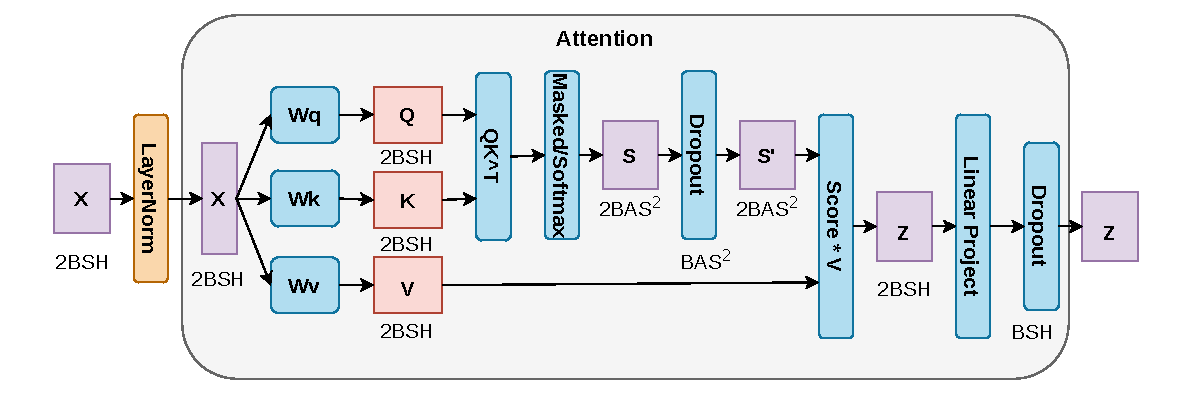
\includegraphics[width=0.85\linewidth]{recomputation_attention.pdf}
  \caption{注意力子层中间激活示意}
  \label{fig:chap4-recomp-attn}
\end{figure}

\paragraph{MLP 子层}：
中间维度 $4H$，第一个线性层的输入为 $2 B S H$，需要保存的输出为 $8 B S H $，经过中间激活后第二个线性层的输入为 $8 B S H$，
最后的 Dropout 层的 mask 矩阵为 $B S H$，合计
\begin{equation}
  N_{\mathrm{mlp}} = 19 B S H.
\end{equation}
图~\ref{fig:chap4-recomp-mlp} 给出了 MLP 子层在 \texttt{None} 情形下需保存的中间激活及其大小。

\begin{figure}[htbp]
  \centering
  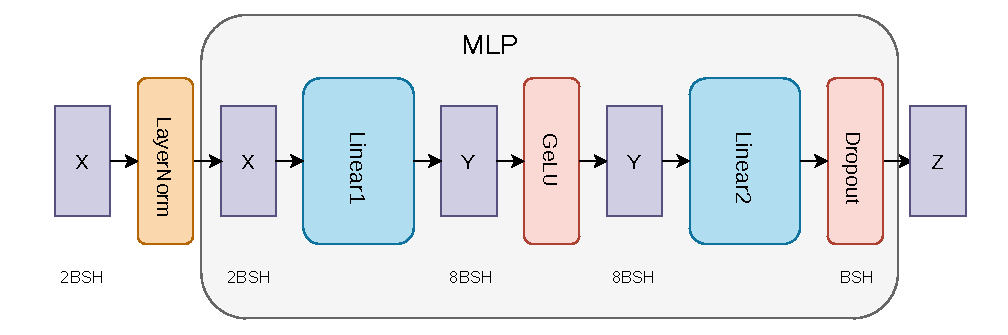
\includegraphics[width=0.85\linewidth]{recomputation_mlp.pdf}
  \caption{MLP 子层中间激活示意}
  \label{fig:chap4-recomp-mlp}
\end{figure}

\emph{两个 LayerNorm}（注意力前、MLP 前）各保存输入 $2 B S H$，合计
\begin{equation}
  N_{\mathrm{ln}} = 4 B S H.
\end{equation}

于是，不采用重计算时单层需保存的中间激活总量为
\begin{equation}
  N_{\mathrm{None}} = N_{\mathrm{attn}} + N_{\mathrm{mlp}} + N_{\mathrm{ln}} = 34 B S H + 5 B A S^2.
\end{equation}
其中 $5 B A S^2$ 项随序列长度平方增长，可能成为长序列场景下中间激活显存的主要来源。

\textbf{（2）选择重计算（\texttt{selective}）。} 仅对指定子模块做重计算：前向只保存该子模块的\emph{输入}，反向传播时在子模块内部重新前向传播再反传，
其它未开启重计算的子模块仍按 \texttt{None} 情形完整保存中间激活。
以仅对 \texttt{core\_attn} 开启选择重计算为例，注意力子层在 \texttt{None} 情形下需要 $N_{\mathrm{attn}} = 11 B S H + 5 B A S^2$ 大小的显存空间来存储中间激活值；
对 \texttt{core\_attn} 做选择重计算之后，Attention 块内部的中间激活（$QK^{\top}$、softmax 及其 dropout mask 矩阵等）都不再常驻显存，
只保留该子模块的输入张量（层输入和 LN 输出）以便在反向传播重新计算注意力块本身；
MLP 子层与两个 LayerNorm 的激活仍按照 $N_{\mathrm{mlp}}$ 与 $N_{\mathrm{ln}}$ 的代价保存，因此整层的线性部分从 $34 B S H + 5 B A S^2$ 约减少为 $23 B S H$。

若在此基础上进一步对 \texttt{mlp} 开启选择重计算，则 MLP 内部的 $19 B S H$ 激活也改为在反向传播时重算，只需要让输入的张量常驻显存，此时需要保存的中间激活总量进一步降低为 $6 B S H$。
再将 \texttt{layernorm} 纳入 \texttt{recompute\_modules} 时，其输出在前向结束后同样可以丢弃，仅保留必要的输入，需要保存的中间激活总量进一步降低为 $4 B S H$。
为便于与 \texttt{None} 情形直观对比，本文用
\begin{align}
  N_{\mathrm{selective}}^{\mathrm{core\_attn}} &= 23 B S H, \\
  N_{\mathrm{selective}}^{\mathrm{core\_attn+mlp}} &= 6 B S H, \\
  N_{\mathrm{selective}}^{\mathrm{core\_attn+mlp+ln}} &= 4 B S H.
\end{align}
来表示选择不同重计算模块下需要存储的中间激活占据的显存总量。
与 \texttt{None} 相比，选择重计算策略去掉了注意力主体与 MLP 主体中的大部分常驻中间激活，仅保留子模块边界的输入张量，显存开销的孔家复杂度由 $O(B S H + B A S^2)$ 降为 $O(B S H)$。

\textbf{（3）整层重计算（\texttt{full}）。} 以整层为重计算单元：前向只保存层输入 X，反向时整层重新前向传播再反向传播计算梯度。
故
\begin{equation}
  N_{\mathrm{full}} =2 B S H.
\end{equation}
这种情况下的显存占用最小，但反向时需重算整层前向，计算开销最大。

表~\ref{tab:chap4-activation} 汇总了不采用重计算、选择重计算与整层重计算时单层需保存的中间激活总量。

\begin{table}[htbp]
  \centering
  \caption{单层 Transformer 中间激活量}
  \label{tab:chap4-activation}
  \small
  \renewcommand{\arraystretch}{1.5}
  \setlength{\tabcolsep}{4pt}
  \begin{tabular}{@{}p{2.5cm}p{4.2cm}p{5.8cm}@{}}
    \toprule
    策略 & 需保存的激活（元素个数） & 说明 \\
    \midrule
    \texttt{None} & $34 B S H + 5 B A S^2$ & 整层所有中间激活均常驻 \\
    \hdashline
    \texttt{selective} [\texttt{core\_attn}] & $23 B S H$ & 仅注意力内部重算，MLP 与 LN 仍常驻 \\
    \hdashline
    \texttt{selective} [\texttt{core\_attn}, \texttt{mlp}] & $6 B S H$ & 注意力与 MLP 内部重算，仅边界与 LN 常驻 \\
    \hdashline
    \texttt{selective} [\texttt{core\_attn}, \texttt{mlp}, \texttt{layernorm}] & $4 B S H$ & 三者均重算，仅两个子模块边界的输入常驻 \\
    \hdashline
    \texttt{full} & $2 B S H$ & 仅保存层输入，反向时整层重算 \\
    \bottomrule
  \end{tabular}\\
  \renewcommand{\arraystretch}{1.0}
  \vspace{2pt}
\end{table}

\subsection{异构重计算策略设计}
\label{sec:HR-MMoH-design}

在 MMoH 已完成的流水线划分与设备映射基础上，HR-MMoH 的异构重计算核心思想是：\emph{为每个流水级（或每台计算设备）根据其显存上限以及算力，独立配置重计算粒度与子模块集合}，
使显存压力大的流水级采用更激进的检查点以降低 OOM风险，显存压力小的流水级采用较保守的配置以减少不必要的重计算开销，从而在满足显存约束的前提下最小化迭代时间并最大化 GPU 利用率。


\paragraph{输入与约束。}
在 MMoH 规划器已完成模型划分与设备映射的前提下，记流水线并行度为 $S$，流水级索引为 $s \in \{1,\ldots,S\}$，
流水级 $s$ 映射至设备 $d_s$。记设备 $d_s$ 的显存容量上界为 $M_s$，相对计算能力系数为 $C_s$（可由该设备 FLOPs 或实测单流水级迭代时间经归一化得到）。
流水级 $s$ 由若干模型块构成；其在前向与反向传播阶段的激活显存峰值及重计算开销由该流水级所采用的检查点配置 $\theta_s$ 唯一确定。
配置 $\theta_s$ 的取值为：\texttt{recompute\_granularity} $\in \{\texttt{None}, \texttt{full}, \texttt{selective}\}$；
当为 \texttt{full} 时还需指定 \texttt{recompute\_method} 与 \texttt{recompute\_num\_layers}，
当为 \texttt{selective} 时则指定 \texttt{recompute\_modules} 子模块列表。形式化地，约束条件为：$\forall s$，
在配置 $\theta_s$ 下流水级 $s$ 的激活显存峰值不超过 $M_s$（可保留安全余量）；优化目标为最小化单次训练迭代时间，
即 $\min \max_s T_s$，其中 $T_s$ 表示流水级 $s$ 在配置 $\theta_s$ 下前向、重计算与反向阶段耗时之和（含流水级间通信）。

\paragraph{问题求解。}
本文采用基于剖析（profiling）的配置生成策略。对每一流水级 $s$，在与其对应的代表设备上预先测量不同 $\theta_s$ 下的激活显存占用与单流水级执行时间 $T_s$；在满足显存约束的可行配置集中，为流水级 $s$ 选取使 $T_s$ 较小且与相邻流水级时间较为均衡的配置，以降低瓶颈流水级对整体迭代时间的主导程度。策略可归纳为两类情形：（1）\emph{显存紧张}的流水级：优先采用 \texttt{full} + \texttt{uniform} 并取较小的 \texttt{recompute\_num\_layers}，或 \texttt{selective} 并采用较完整的 \texttt{recompute\_modules}（如 \texttt{[core\_attn, mlp, layernorm]}），以降低激活显存峰值、避免 OOM；（2）\emph{显存充裕而算力或通信紧张}的流水级：采用 \texttt{None}，或 \texttt{selective} 且仅 \texttt{[core\_attn]}，或 \texttt{full} + \texttt{block} 且较小的 \texttt{recompute\_num\_layers}，以减少不必要的重计算与同步开销。实现上，在 MMoH 规划器输出流水级划分与设备映射之后，由 HR-MMoH 配置模块为各流水级生成对应的 \texttt{TransformerConfig} 参数（或等价的环境变量/配置文件），各训练进程（rank）在初始化时加载其所属流水级的配置，从而在保持 Megatron 单卡前向/反向语义不变的前提下，实现按流水级异构的重计算。

\paragraph{与 MMoH 的协同。}
HR-MMoH 以 MMoH 给出的流水级划分与设备映射为输入，二者形成层次化协作：若在统一检查点策略下某流水级仍出现显存溢出，可将该信息反馈至 MMoH 规划器（例如在显存约束中提高该流水级的权重，或对该流水级进行更细粒度的块划分），从而实现划分与显存配置的迭代优化。第三章所述的提前终止调度器在冻结流水级上省略反向计算与梯度通信，与各流水级独立的检查点配置无冲突：冻结流水级可采用较保守的检查点策略以节省计算，非冻结流水级则按显存与算力约束进行均衡配置。

\section{实验验证}
\label{sec:HR-MMoH-exp}

本节从实验设置、实验结果与实验分析三方面对 HR-MMoH 的设计动机与配置思路进行说明；完整端到端实现及与 MMoH 的联合吞吐对比可作为后续工作深化。

\subsection{实验设置}

\paragraph{平台与配置思路验证。}
实验环境与第三章 MMoH 实验一致，采用两种异构集群（Cluster-S、Cluster-L）及两种 MLLM（MLLM-3B、MLLM-12B）。为验证“按流水级差异化配置”的合理性，对 MMoH 划分得到的各流水级进行显存与耗时剖析：在每流水级对应的设备上，分别测量 \texttt{recompute\_granularity=None}、\texttt{selective} 且 \texttt{recompute\_modules=[core\_attn]}、\texttt{[core\_attn, mlp]}、\texttt{[core\_attn, mlp, layernorm]} 以及 \texttt{full} + \texttt{uniform} 且不同 \texttt{recompute\_num\_layers} 下的激活峰值与单流水级前向+反向时间（含重算）。据此可得到各流水级在满足显存约束下的可选配置集合及对应的 $T_s$，用于验证显存紧张流水级与充裕流水级在“最省显存”与“最少重算”配置上的差异是否显著，以及按流水级赋配置后各 $T_s$ 是否更均衡。

\paragraph{对比与指标。}
重计算的对比基线为全局统一配置：所有流水级不采用重计算，记为\texttt{no-recomp}；所有流水级采用相同的 \texttt{full recomputation}，即在前向传播中丢弃所有的中激活值，记为\texttt{full}；
所有流水级采用相同的 \texttt{selective} + \texttt{[core\_attn]} 或 \texttt{[core\_attn, mlp, layernorm]}（记为 \texttt{select-1} 与 \texttt{select-2}）。
指标包括：（1）各流水级在满足显存不溢出条件下的显存占用峰值与单流水级耗时 $T_s$；（2）完整训练循环的训练吞吐（\texttt{samples/s} 和迭代时间\texttt{s/iteration}。

\subsection{实验结果}

在 MMoH 对 MLLM-3B / MLLM-12B 的划分结果上，对各流水级进行上述剖析后可观察到：显存相对紧张流水级（如承载 LLM 中段或大 block 的流水级）在 \texttt{recompute\_granularity=None} 或仅 \texttt{[core\_attn]} 时易接近或超出设备显存上限，需采用 \texttt{[core\_attn, mlp, layernorm]} 或 \texttt{full} + \texttt{uniform} 方能安全训练；而显存充裕流水级（如部分编码器或投影层所在流水级）采用 \texttt{[core\_attn, mlp, layernorm]} 会带来不必要的重算，单流水级耗时 $T_s$ 明显增加。按流水级赋予差异化配置（显存紧张流水级用较激进检查点，充裕流水级用较保守检查点）后，各流水级 $T_s$ 的方差较 Uniform-1 / Uniform-3 有所下降，迭代时间 $\max_s T_s$ 在多数场景下优于或接近“为照顾最紧张流水级而全局采用 Uniform-3”的配置，说明异构感知的配置策略在理论上能够兼顾显存安全与负载均衡。完整训练循环下的吞吐对比有待在 HR-MMoH 与 Megatron/MMoH 的深度集成实现后进一步报告。

\subsection{实验分析}

\paragraph{显存—算力权衡。}
异构集群上各流水级显存与算力分布不均，统一配置要么为防 OOM 而整体偏保守导致重算过多，要么为减重算而整体偏激进导致瓶颈流水级 OOM。按流水级配置后，可在满足各流水级显存约束的前提下，将“重算预算”更多分配给显存紧张、算力相对充裕的流水级，从而在系统层面降低迭代时间。

\paragraph{与 MMoH 划分的配合。}
MMoH 的复合粒度与冻结感知划分已使各流水级负载趋于均衡；HR-MMoH 在此基础上对显存维度做细粒度调节，二者结合可形成“划分—调度—显存优化”的闭环。未来工作可将 HR-MMoH 的配置搜索与 MMoH 的整数规划联合建模，或采用分层决策：先由 MMoH 确定划分与映射，再由 HR-MMoH 模块为各流水级输出推荐配置并可选地反馈显存不足信息以触发重新划分。

\section{本章小结}
\label{sec:HR-MMoH-summary}

本章在 MMoH 的异构流水线划分与提前终止调度基础上，针对显存受限流水级仍可能 OOM、而现有重计算策略多采用全局统一配置难以兼顾显存与效率的问题，
介绍了 HR-MMoH 的异构重计算思路。
首先系统梳理了 Megatron-LM 的重计算配置参数（\texttt{recompute\_granularity}、\texttt{recompute\_method}、\texttt{recompute\_num\_layers}、\texttt{recompute\_modules} 等）
及其 \texttt{full/selective} 粒度与层级划分方式，并指出其在同构假设下的局限；随后给出了 HR-MMoH 的设计要点：以各流水级显存上限、算力为约束，为各流水级独立配置重计算粒度与子模块集合，通过基于剖析的配置策略在满足显存不溢出的前提下最小化迭代时间并平衡各流水级负载，并与 MMoH 划分及提前终止调度器协同。
实验部分说明了配置思路的验证方式与预期效果，并指出完整端到端实现与联合吞吐对比可作为后续工作。
HR-MMoH 与第三章的 MMoH 共同构成“划分—调度—显存优化”的联合优化框架，为异构 GPU 集群上 MLLM 的高效训练提供了显存维度的补充手段。

\chapter{总结与展望}

本章对全文工作进行总结，概括主要创新点，归纳研究局限，并从若干研究问题展望未来工作。

\section{全文工作总结}

本文围绕"面向异构 GPU 集群的多模态大语言模型并行训练技术"这一主题，针对实际环境中普遍存在的设备异构与 MLLM 的模块异构、分阶段冻结训练等特性，从\emph{模型划分与流水线调度}与\emph{重计算优化}两个层面开展了研究，提出了 MMoH 与 HR-MMoH 两套方法，并在异构集群上进行了实验验证。下文概括主要创新点。

\subsection{主要创新点}

本文的主要创新点可归纳为以下两方面。

\textbf{（1）MMoH：面向异构 GPU 集群的多模态大语言模型高效混合并行框架。}

针对异构集群上 MLLM 训练时存在的负载不均衡、资源利用率低以及冻结场景下冗余计算与通信等问题，本文提出了 MMoH 框架。其创新点包括：\emph{需求驱动的设备拓扑识别}，根据 MLLM 各模块的计算与显存需求趋势与异构设备的算力—显存供给进行匹配，筛选候选设备拓扑，使需求与供给在趋势上一致。\emph{复合粒度模型抽象}，针对编码器、投影层与 LLM 基座的结构差异，采用多级粒度将模型重组为模型块列表（编码器按子模块合并、LLM 按注意力/FFN 子层拆分），在划分复杂度与负载均衡之间取得折中。\emph{冻结感知的模型划分}，将块到阶段的分配形式化为整数规划问题，在满足显存与主阶段约束下最小化迭代时间，且目标函数显式依赖各阶段的冻结状态，从而随训练阶段动态调整划分策略。\emph{提前终止调度器}，在 1F1B 等流水线调度基础上，识别从首端开始的连续冻结阶段并对其省略反向计算与流水级间通信，在不影响模型收敛性的前提下提升吞吐。在两种异构集群（Cluster-S、Cluster-L）与两种规模 MLLM（MLLM-3B、MLLM-12B）上的实验表明，MMoH 在 no-freeze、freeze-encoder、freeze-llm、freeze-both 四种场景下相对 Megatron-LM、Whale、Espresso 均可取得最高吞吐，最高可达约 1.77$\times$ 加速，且提前终止调度器在冻结场景下可带来约 8\%--19\% 的额外增益，并具有良好的可移植性。

\textbf{（2）HR-MMoH：面向异构设备与异构模型的重计算策略优化。}

针对现有重计算策略在同构假设下采用全局统一配置、难以在异构集群上同时兼顾显存安全与计算效率的问题，本文在 MMoH 的划分与调度基础上，提出并实现了 HR-MMoH 的异构重计算方法。HR-MMoH 使各流水级根据自身显存与算力条件采用差异化的重计算粒度（如 full/selective）与子模块选择，在降低 OOM 风险的同时减少多余重算、平衡流水级负载，与 MMoH 形成 "划分—调度—重计算" 的联合优化。第四章在更大批次大小与更长序列长度的实验下证明，HR-MMoH 在 no-freeze、freeze-encoder、freeze-llm、freeze-both 四种冻结场景中均取得最高吞吐，相对 Espresso 的迭代时间缩短约 6.1\%--23.1\%，在 Whale 可训练的三种冻结场景中缩短约 11.0\%--40.6\%。这说明按流水级差异化配置能够系统性优于全局统一策略，并验证了与 MMoH 协同优化的有效性。

综上，本文在异构 GPU 集群上 MLLMs 并行训练这一方向上，从\emph{划分与调度}与\emph{显存优化}两条线给出了系统性的方法设计与实验支撑，为实际部署中的混合集群与分阶段训练场景提供了可参考的技术路径。

\section{局限性及未来工作展望}

结合前文全文总结，本节先归纳研究局限，再围绕后续研究的核心问题与思路作简要展望。

\subsection{研究局限性}

本研究仍存在以下局限，亦是后续工作的重要出发点。

规划器中的整数规划求解在模型层数与设备数较大时可能面临组合爆炸，当前采用启发式或现有求解器在有限时间内求近似解，最优性保证与可扩展性仍有提升空间；实验仅在两种规模的 MLLM（3B、12B）与两种异构集群配置上进行，对更大规模模型（如 70B+）、更多代际与型号混合的集群以及更长序列、更多模态的 MLLMs 的泛化能力有待进一步验证。

尽管第四章已完成端到端实验并验证了按流水级异构重计算的收益，当前策略搜索仍以启发式与剖析驱动为主，候选配置空间、搜索顺序与回退机制依赖经验设计，尚未给出更强的最优性保证与复杂度分析；实验主要在 Cluster-L 与 MLLM-12B 上开展，对更大规模模型、更复杂模型结构（如 MoE 模型）及更长上下文设定下的鲁棒性仍需补充；此外，HR-MMoH 与 MMoH 的联合优化目前仍采用"先划分、后配置重计算"的分层流程，尚未形成统一目标下的联合求解框架。

当前工作主要针对视觉—语言类 MLLM 与 NVIDIA GPU 生态，对音频、视频等多模态输入、以及 AMD、国产 GPU 等异构硬件与软件栈的适配与评估尚未涉及；与专家并行、上下文并行等已有技术的协同优化仍有扩展空间。

\subsection{未来研究工作}

基于上述局限，后续研究可沿以下两条线索推进。

\textbf{（1）划分与重计算的联合求解。}
本文采用"先由 MMoH 求解划分与设备拓扑，再由 HR-MMoH 为各流水级搜索重计算配置"的分层流程。该流程存在循环依赖：划分决定各流水级的层分配与显存余量，进而影响可选的重计算配置与各流水级耗时；而重计算配置改变后各流水级的实际耗时又反过来改变最优划分。当前分层求解无法捕捉这种耦合，可能遗漏"不同划分 + 不同重计算组合"下迭代时间更低的方案。一种可行思路是将重计算配置作为决策变量引入第三章的整数线性规划，把重计算带来的额外前向开销纳入迭代时间目标，使划分与重计算在同一目标下联合求解；或采用交替优化——固定重计算求划分，再固定划分更新重计算——并分析其收敛性。此方向的核心在于量化分层流程的次优性来源及其量级，为判断是否值得引入联合求解提供依据。

\textbf{（2）提前终止调度向新型流水线机制的扩展。}
第三章的提前终止调度器与迭代时间的推导均建立在 1F1B 调度之上。近年提出的 ZeroBubble\cite{zerobubble2024} 将反向拆分为"对输入的梯度"与"对参数的梯度"两个独立阶段，通过 1F1B1W 调度将后者与下一 micro-batch 的前向重叠以压缩气泡；DualPipe\cite{dualpipe2025} 则采用双向 micro-batch 流动实现前反向交织。
这两类调度改变了流水级间的依赖结构：冻结流水级不需要计算对参数的梯度，但对输入的梯度能否被提前终止剪枝，取决于后续流水级在新调度下的依赖关系是否与 1F1B 一致。
在上述新调度框架下重新推导冻结前缀的可剪枝条件与迭代时间收益，并验证其与 HR-MMoH 按流水级差异化重算的兼容性可作为下一步研究工作。
若成功推广，可在进一步压缩气泡的同时保留冻结前缀剪枝的收益，使 MMoH 框架适用于更广泛的工程实践。

综上所述，本文在面向异构 GPU 集群的 MLLMs 并行训练策略方面取得了阶段性成果；后续宜在划分与重计算的联合求解、以及提前终止向新型流水线调度的扩展两个方向上继续推进，为异构环境下 MLLMs 训练的进一步优化提供方法与理论支撑。


%%% Local Variables:
%%% mode: latex
%%% TeX-master: "../thesis"
%%% End:

\begin{ack}

攻读硕士学位期间，本论文的完成离不开各位老师、同学与家人的关心与支持，在此谨致谢忱。

\end{ack}


\cleardoublepage
\phantomsection
\addcontentsline{toc}{chapter}{参考文献}
\bibliographystyle{bstutf8}
\bibliography{ref/refs}

\input{data/resume}    %在学期间成果
% \begin{reviewinfo}

	\newlength{\reviewtablewidth}
	\newlength{\reviewtableinnerwidth}
	\newcolumntype{R}[1]{m{#1\reviewtableinnerwidth}}
	\newcommand{\reviewhead}[1]{\parbox[c][34pt][c]{\linewidth}{\centering \hei #1}}
	\newcommand{\reviewheadmulti}[2]{\parbox[c][34pt][c]{\linewidth}{\centering \hei #1\\[-4pt]\hei #2}}
	\newcommand{\reviewcell}[1]{\parbox[c][42.5pt][c]{\linewidth}{\centering #1}}
	\begin{table}[tbh]
		\centering
		{\wuhao
		\setlength{\tabcolsep}{0.5pt}
		\setlength{\reviewtablewidth}{\linewidth}
		\setlength{\reviewtableinnerwidth}{\dimexpr\reviewtablewidth-18\tabcolsep-10\arrayrulewidth\relax}
		% word模板中原始的比例如下
		% 为显示更美观，针对职称（副研究员）和导师类型（非导师），微调了比例
		% \begin{tabular}{|R{0.075}|R{0.103}|R{0.103}|R{0.075}|R{0.224}|R{0.128}|R{0.078}|R{0.146}|R{0.064}|}
		\begin{tabular}{|R{0.075}|R{0.103}|R{0.113}|R{0.085}|R{0.21}|R{0.108}|R{0.078}|R{0.12}|R{0.104}|}
			\hline
			\reviewhead{序号} & \reviewhead{评阅人} & \reviewhead{职称} & \reviewheadmulti{导师}{类型} & \reviewhead{工作单位} & \reviewhead{评分} & \reviewheadmulti{答辩}{建议} & \reviewhead{熟悉程度} & \reviewhead{备注} \\
			\hline
			\reviewcell{1} & \reviewcell{王晓东} & \reviewcell{研究员} & \reviewcell{博导} & \reviewcell{国防科技大学} & \reviewcell{83} & \reviewcell{A} & \reviewcell{比较熟悉} & \reviewcell{} \\ \hline
			\reviewcell{2} & \reviewcell{李荣春} & \reviewcell{研究员} & \reviewcell{硕导} & \reviewcell{国防科技大学} & \reviewcell{90.3} & \reviewcell{B} & \reviewcell{比较熟悉} & \reviewcell{\mbox{}} \\ \hline
			\reviewcell{3} & \reviewcell{张博锋} & \reviewcell{正高级工程师} & \reviewcell{硕导} & \reviewcell{飞腾信息技术有限公司} & \reviewcell{85.45} & \reviewcell{A} & \reviewcell{比较熟悉} & \reviewcell{行业专家} \\ \hline
			\reviewcell{4} & \reviewcell{专家四} & \reviewcell{} & \reviewcell{} & \reviewcell{} & \reviewcell{84} & \reviewcell{B} & \reviewcell{比较熟悉} & \reviewcell{校级评阅} \\ \hline
			\reviewcell{5} & \reviewcell{专家五} & \reviewcell{} & \reviewcell{} & \reviewcell{} & \reviewcell{88} & \reviewcell{A} & \reviewcell{有深入了解} & \reviewcell{校级评阅} \\ \hline
		\end{tabular}}
	\end{table}
	
	\wuhao{
	\noindent \textbf{说明}：
	
		1. 答辩建议选项包括4个：“A同意直接答辩”、“B同意修改后答辩”、“C须作较大\linebreak[4]修改后复评”、“D不同意答辩”。
	
		2. 熟悉程度选项包括3个：“有深入了解”、“比较熟悉”、“一般了解”。
	\\
	}
	
	\end{reviewinfo} %公开评阅信息
% \begin{defensecommittee}

\begin{table}[tbh]
	\centering
	\begingroup
	\setlength{\tabcolsep}{12pt}%
	\renewcommand{\arraystretch}{2.1}%
	% p 列顶对齐；m 列在格内上下居中。X 列默认等价于 p，改为 m 才垂直居中：
	\renewcommand{\tabularxcolumn}[1]{>{\centering\arraybackslash}m{#1}}%
	\begin{tabularx}{\linewidth}{|>{\centering\arraybackslash}m{2.6cm}|>{\centering\arraybackslash}m{3cm}|X|>{\centering\arraybackslash}m{2.6cm}|}
		\hline
		\hei{姓名} & \hei{职称} & \hei{\makecell[c]{工作单位}} & \hei{备注} \\
		\hline
		 &  &  &  \\
		\hline
		 &  &  &  \\
		\hline
		 &  &  &  \\
		\hline
		 &  &  &  \\
		\hline
		 &  &  &  \\
		\hline
	\end{tabularx}
	\endgroup
\end{table}

\wuhao{
\noindent \textbf{说明}：\\
1. 请按学院最新要求填写答辩委员会名单；秘书一般不计入委员人数。\\
2. 盲评版、送审版可删去本页或隐去委员信息，以学位办要求为准。\\

\color{red}{
\noindent 提醒（正式成文后删除）：上表为占位示例，请替换为真实信息。
}

}

\end{defensecommittee}
 %答辩委员会
% 最后，需要的话还要生成附录，全文随之结束。
\backmatter

\end{document}
